\chapter{Extended Persistence and Branch Decomposition}
\label{chapter6}

\section{Persistence of Branches}

% In this subsection we will tackle a claim that has been made in the paper that first introduced branch decomposition of contour trees. The claims is the following : "... we define the persistence of a branch to be the greater of its length and the persistence of each of it children. This definition differs from the definition of persistence given in [10] because it takes into consideration the topological obstructions. " \cite{ct-branch-decomp}. In that quote the reference to "[10]" is to the original paper that introduced persistent homology \cite{persistence-original}.

In the original paper the introduces branch decomposition of contour trees make serveral references to topological persistence and persistent homology in defining the persistence of branches.

\begin{itemize}
  \item ". We have tested the approach using topological persistence (that is the difference in function value between a pair of critical points that are simplified) as the main metric for constructing the topological hierarchy"
  \item  "In the next section we will discuss the construction of a hierarchical decomposition based on the persistence of critical point pairs."
  \item "We can now define an order on the branches that allows to extract a contour tree after any number of simplifications in linear time. First, we define the persistence of a branch to be the greater of its length and the persistence of each of it children. This definition differs from the definition of persistence given in [10] because it takes into consideration the topological obstructions. Thus a pair of critical points is never assigned a persistence value that is less than any of its obstructions."
  \item  "Since the branches are sorted by their persistence we always draw the branches with greater persistence first (see Figures 5
and 6)."
\end{itemize}

What is not described however is how the persistence of the branches is derived formally withing the framework of persistent homology as it has been laid out in \cite{persistence-original}. We believe that this is am important addition to the work especially since in the third quote we presented the authors have referenced one paper as "[10]" which is exactly "Topological Persistence and Simplification".

Describing formally the connection between the two in a complete and rigrous manner is beyond the scope of this dissertation. We will however pose and answer one small question that relates branch decomposition and extended persistence. Are the pairs of critical points produces by branch decomposition the same as the pairs of points produced by extended persistence of the zeroth homology? We will demonstrate that they are not will a small counter example. The counter example is based on our familliar w-structures.


\section{Persistence Pairs vs Branch Decomposition Pairs}

Let us first begin with an example data set show in Figure []. Let us call that $X$. The contour tree of this data set is shown in Figure [] and a branch decomposition of this contour tree is shown in Figure []. Note that the global minimum $0$ and the global maximum $8$ cannot be appear in the same branch of any branch decomposition of the contour tree. There is no monotone path between them. There branch decomposition cannot produce the pair $(0, 8)$. According to \cite{ct-branch-decomp}

This is problematic because the extended persistence of $X$ does produce the pair $(0, 8)$ in the zeroth homology. Let us verify that. The ascending filtration of this data set is shown in Figure []. The ascending filtration consists of nine simplical complexes $\{X_1, X_2, ..., X_9\}$. According to our extended persistence computation the pair are $(1, 4)$ and $(0, 8)$. The first pair comes from ordinary persistence. We can see on Figure [] that a component is born in time $1$ and dies in time $4$. The second pair is of the global minimum and global maximum. It comes from extended persistence. To verify this observe that $H_0(X_9) = \mathbb{Z}_2$ because $X_9 = X$ has one connected component.
The next homology group in the sequence is $H_0(X, X^9)$. From the Excision Theorem we have that $H_0(X, X^9) = \overset{\sim}{H}_0(X / X^9)$. However $X / X^9 = X / \{9\} = X$ because quotienting by a single points leaves the complex unchanged. Therefore $H_0(X, X^9) =
\overset{\sim}{H}_0(X)$. We have already explained that $H_0(X) = \mathbb{Z}_2$, so $\overset{\sim}{H}_0(X) = 0$ and consequently $H_0(X, X^9) = 0$. This means that the induced map $i_* : H_0(X_9) \to H_0(X, X^9)$ is the zero map. The conclusion we draw is that the homology class that is born at time $0$ at the global minimum dies at time $8$. Extended persistence produces the pair pair $(0, 8)$.

Note that this is the case for the descending filtration or for that matter for any filtration of any path connected simplicial complex. Let us demonstrate this. Let $M$ be path connected simplicial complex. Then $H_0(M) = \mathbb{Z}_2$. Let $H_0(M, M')$ be any of the groups in the relative sequence where $M'$ is a subcomplex of $M$. By Excision we have that $H_0(M, M') = \overset{\sim}{H}_0(M / M')$. From topology we know that [] a quotient space of a path connected topological space is path connected. Therefore $H_0(M / M') = \mathbb{Z}_2$ and $\overset{\sim}{H}_0(M / M') = 0$ accordingly. We have thus shown that in the extended persistence of a path connected simplicial complex the global minimum pairs with the global maximum.

Here is the summary of our findings.

\begin{itemize}
    \item There is no monotone path between the global minimum and global maximum in the simplicial mesh.
    \item There is no monotone path between the global minimum and global maximum in the contour tree.
    \item No branch decomposition of the contour tree can pair the global minimum and the global maximum.
    \item Extended persistence pairs the global minimum and the global maximum.
\end{itemize}

This counter examples demonstrates that branch decomposition does not yield pairs of critical points that are equivalent to extended persistence. In the next chapter we will discuss what other future question we can pose.

\begin{figure}[h]%
    \centering
    \subfloat[Contour Tree]{{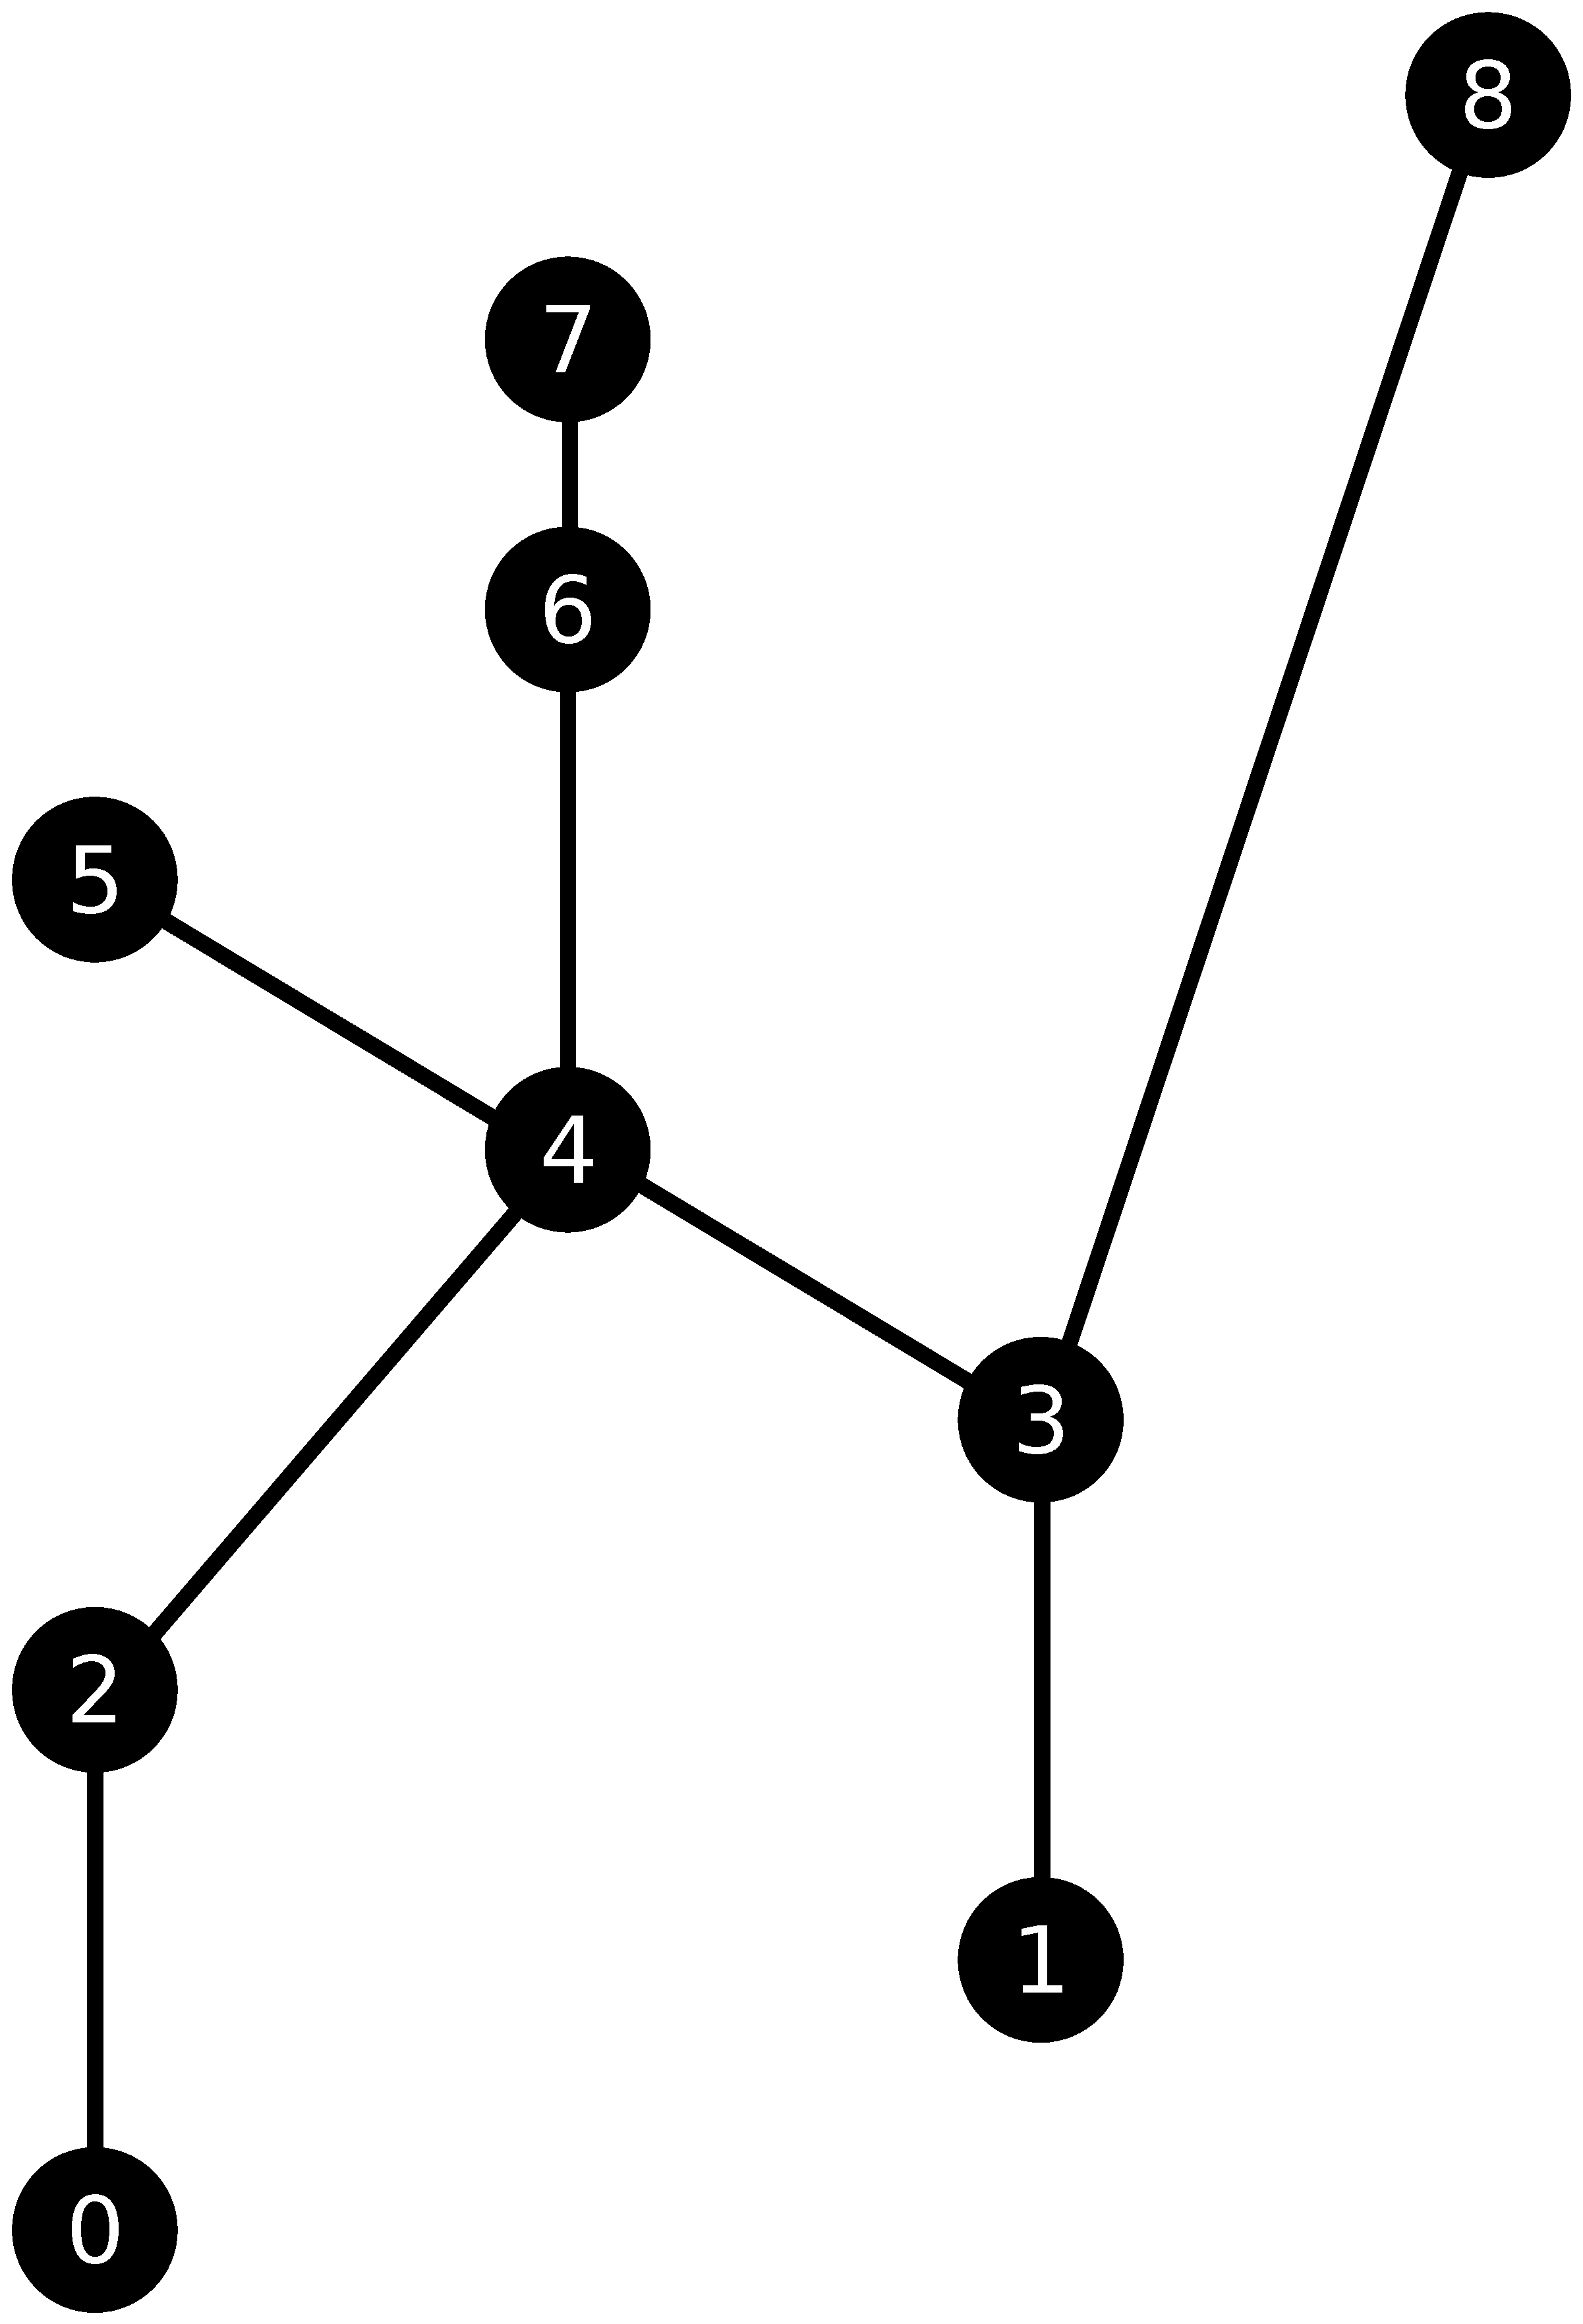
\includegraphics[scale=0.12]{./images/w3x3-contour-tree-new.eps}}}%
    \qquad
    \subfloat[Branch Decomposition]{{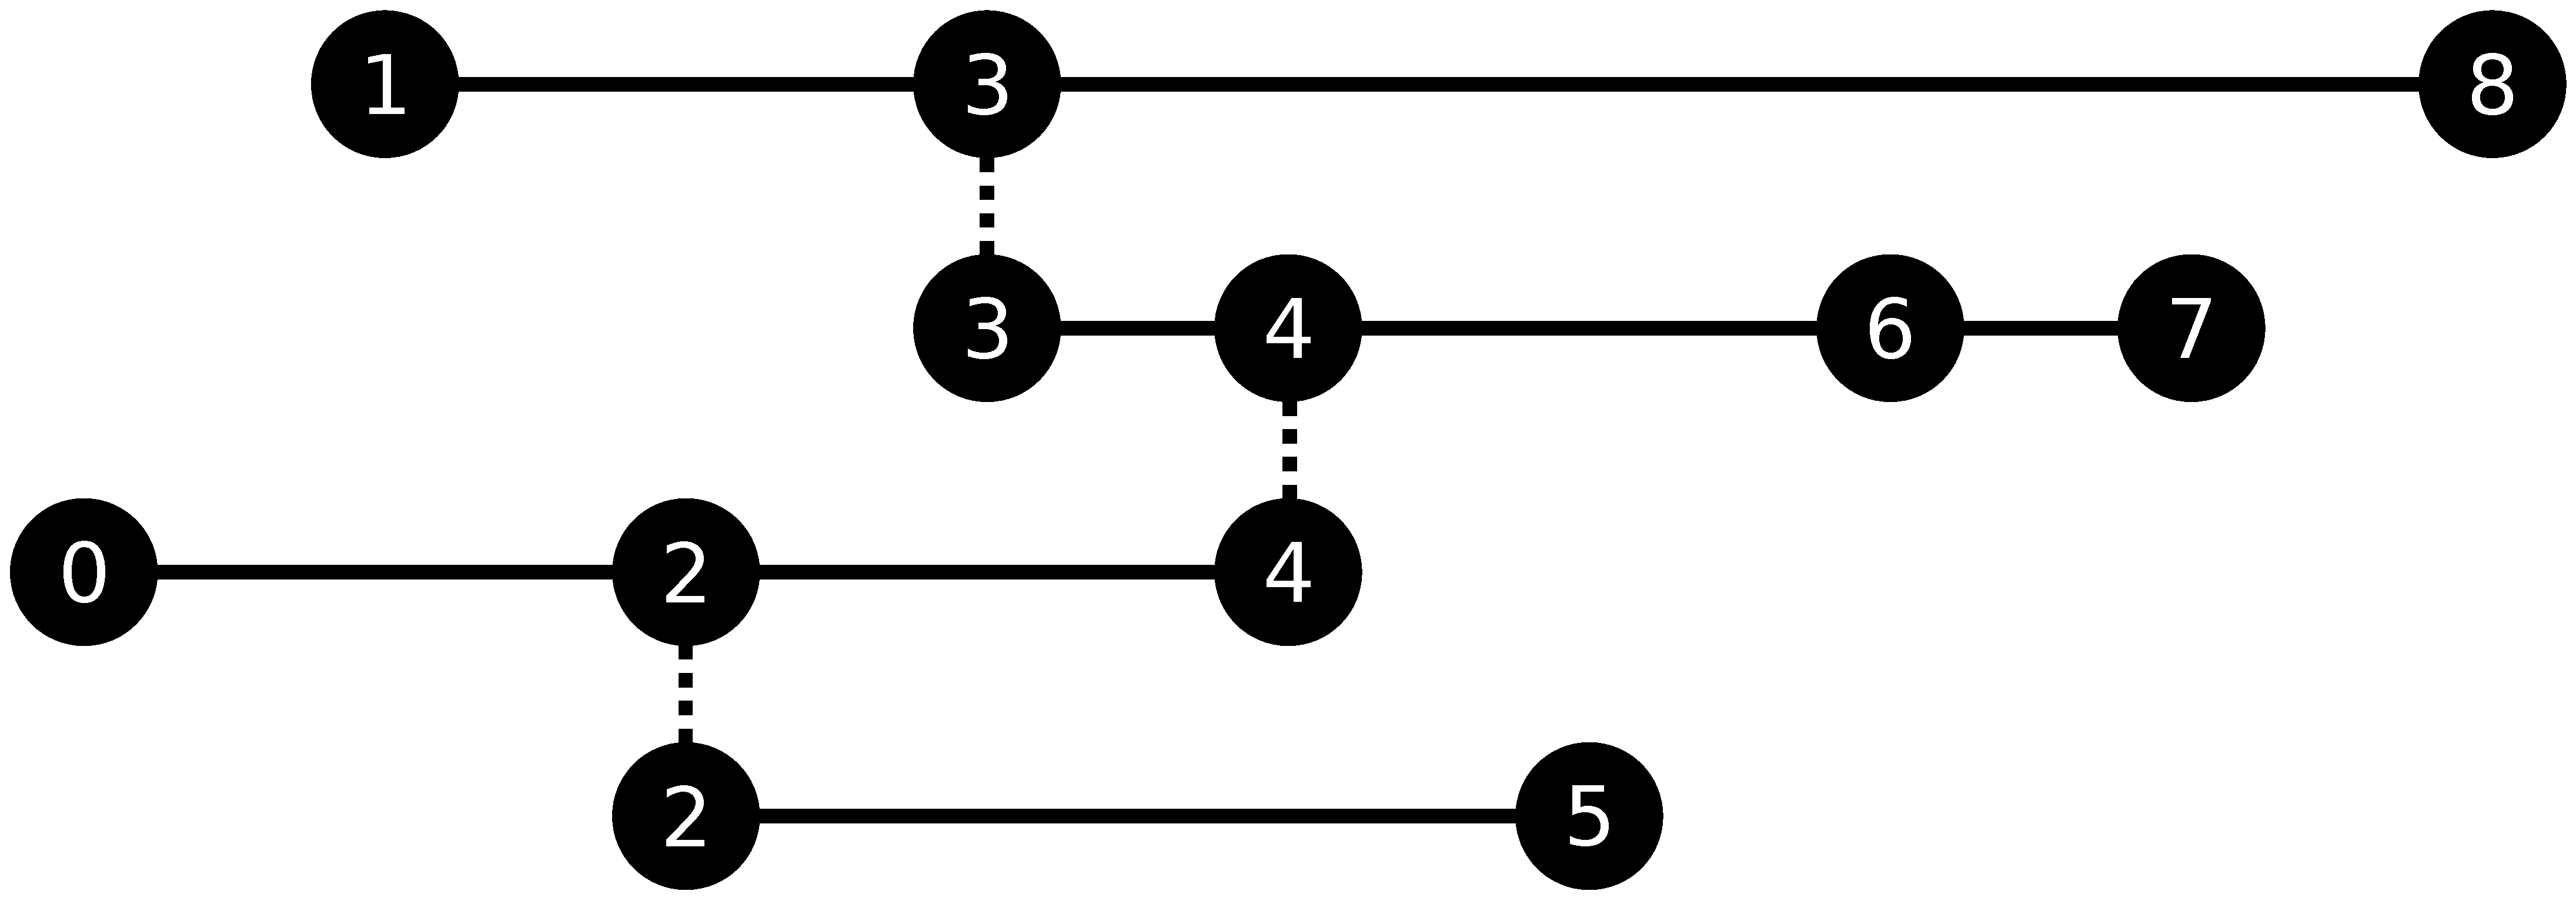
\includegraphics[scale=0.12]{./images/w3x3-contour-tree-decomposition.eps}}}%
    \caption{Branch Decomposition of the contour tree.}%
    \label{fig:example}%
\end{figure}


\begin{figure}[h]%
    \centering
    \subfloat[Join Tree]{{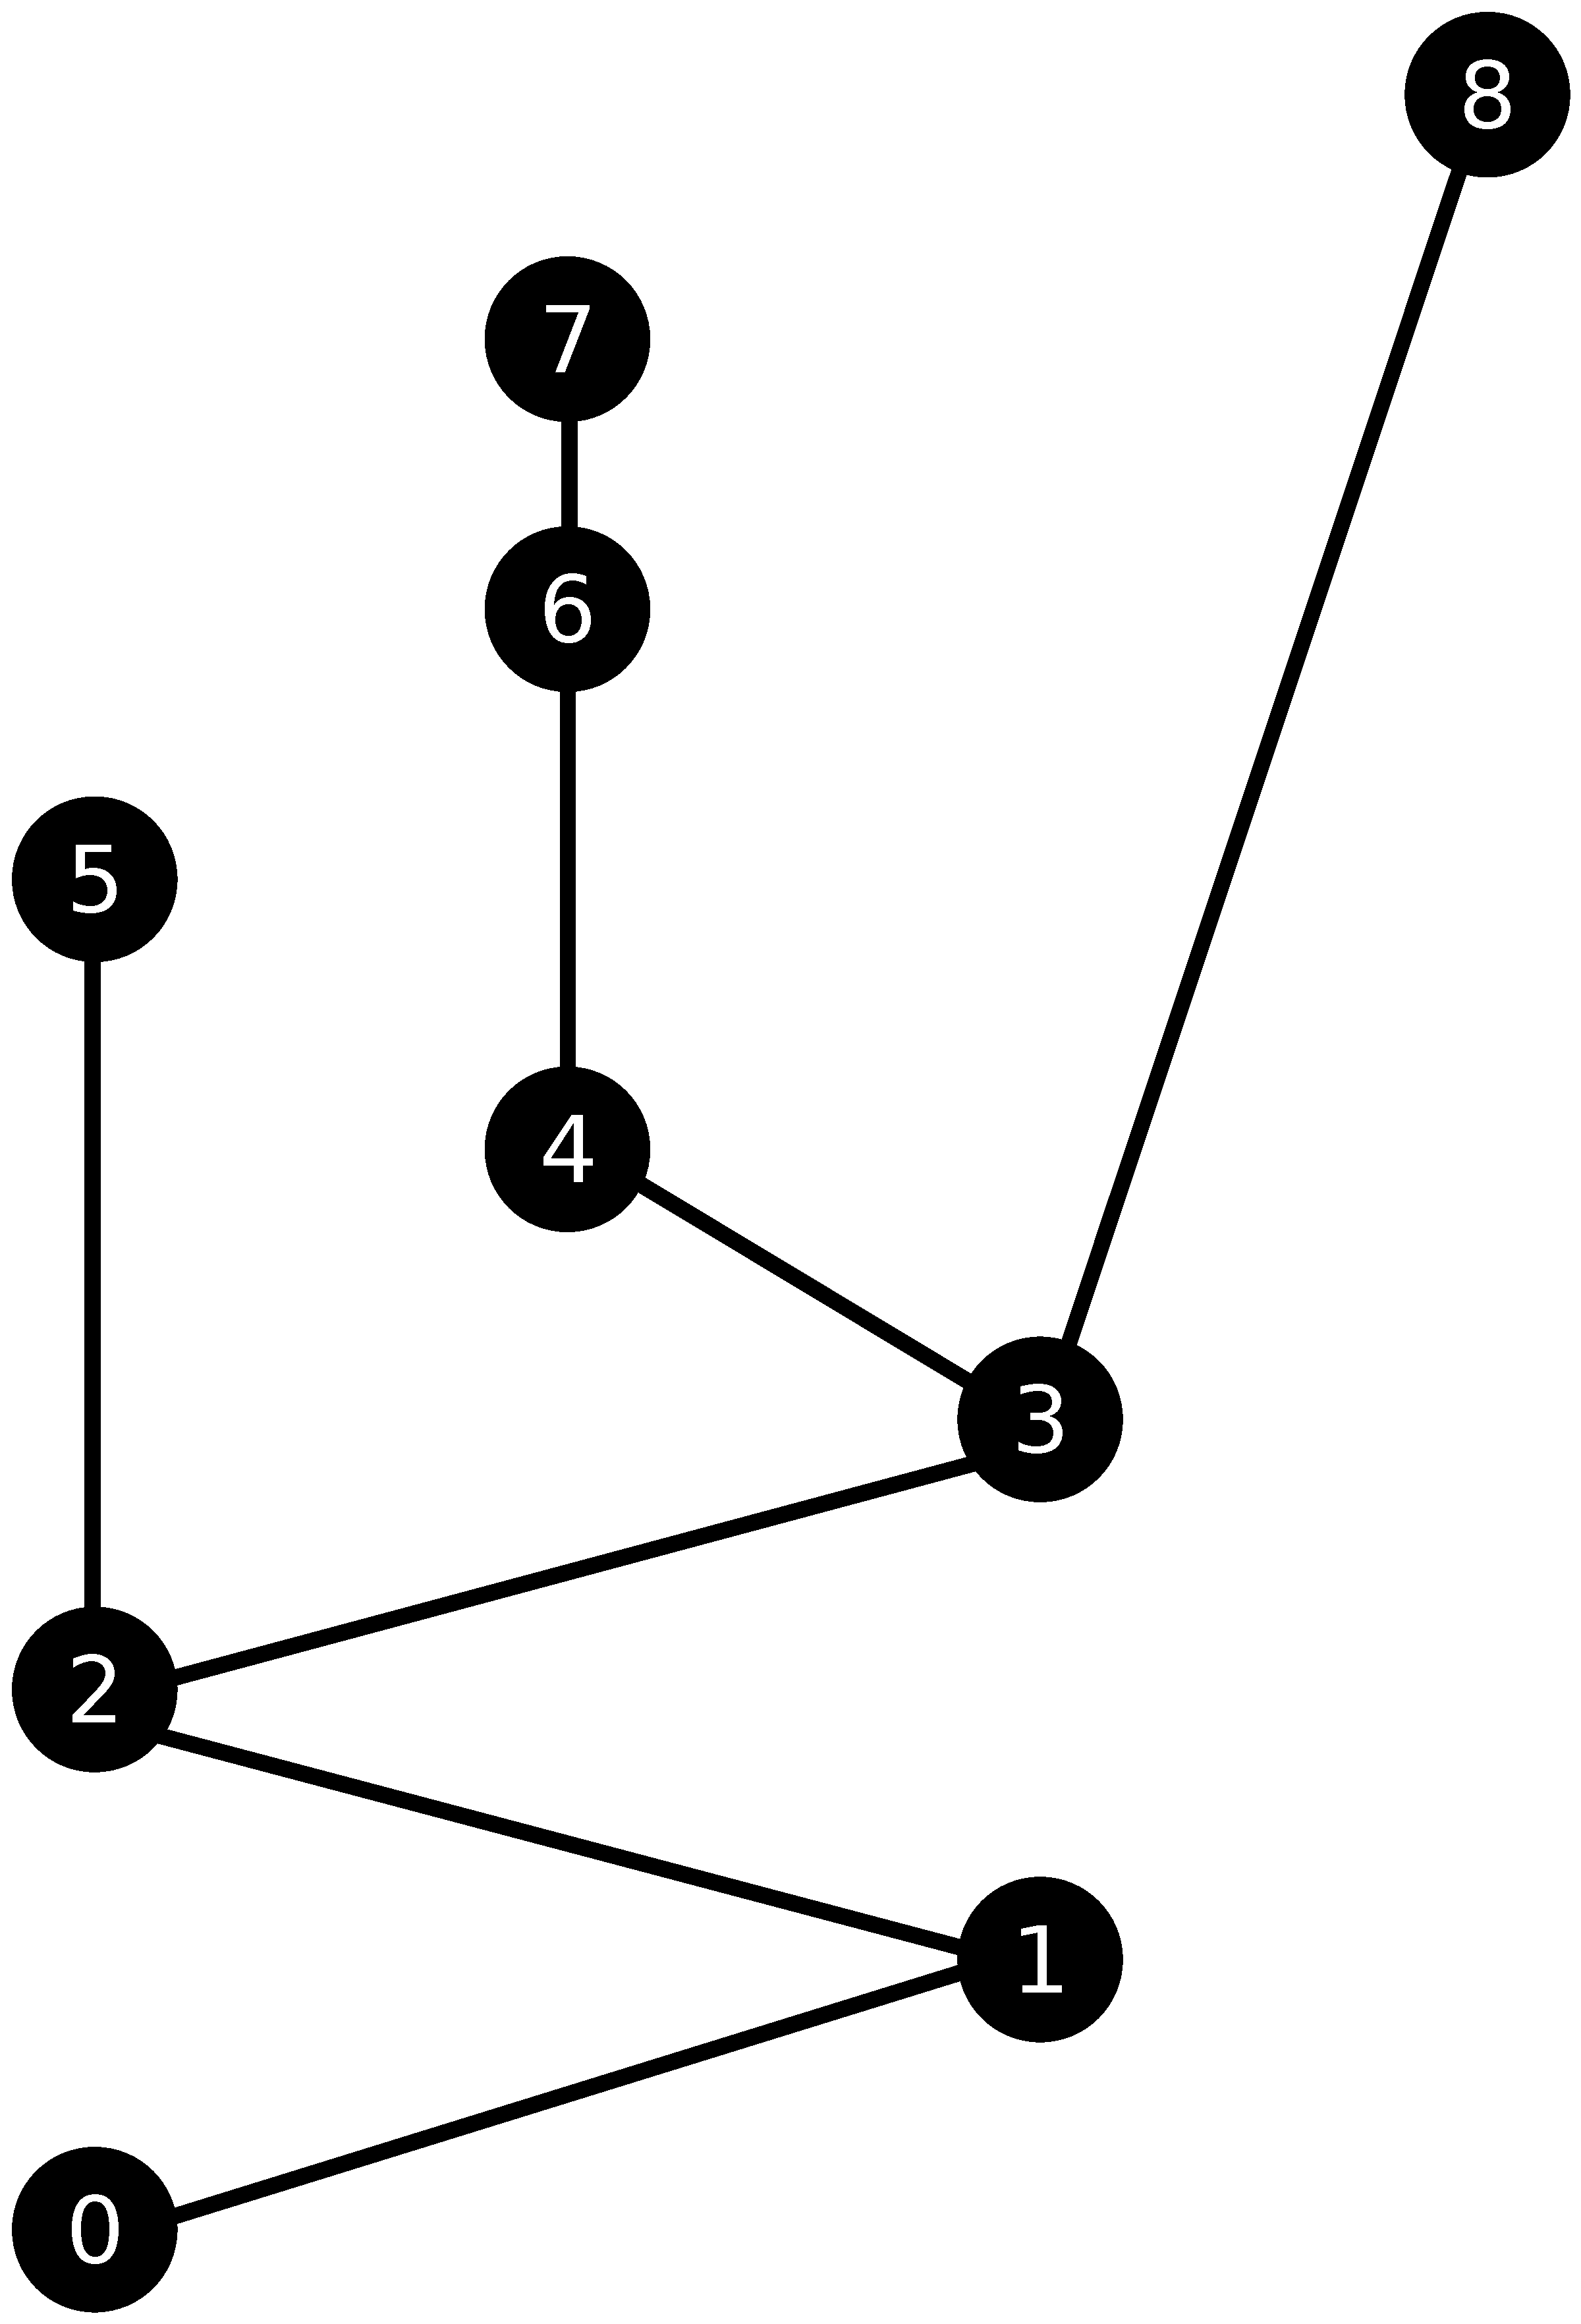
\includegraphics[scale=0.12]{./images/w3x3-join-tree-new.eps}}}%
    \qquad
    \subfloat[Branch Decomposition]{{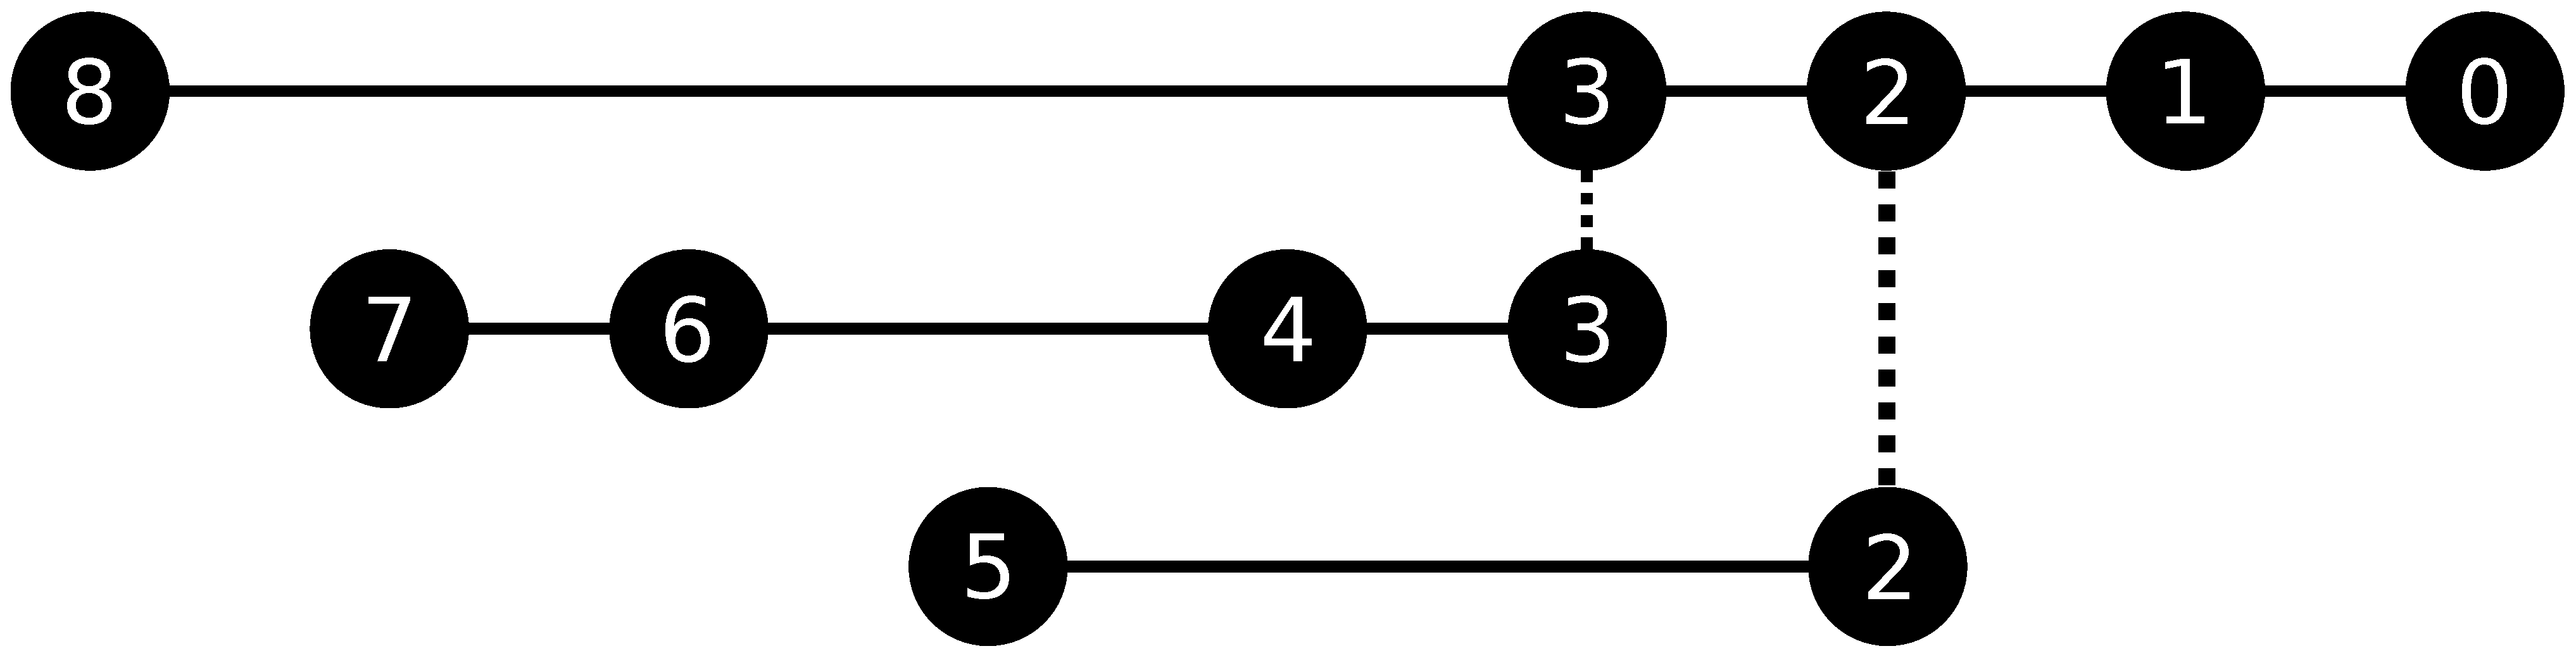
\includegraphics[scale=0.12]{./images/w3x3-join-tree-decomposition.eps}}}%
    \caption{Branch Decomposition of the join tree.}%
    \label{fig:example}%
\end{figure}


\begin{figure}[h]%
    \centering
    \subfloat[Split Tree]{{\includegraphics[scale=0.12]{./images/w3x3-split-tree-new.eps}}}%
    \qquad
    \subfloat[Branch Decomposition]{{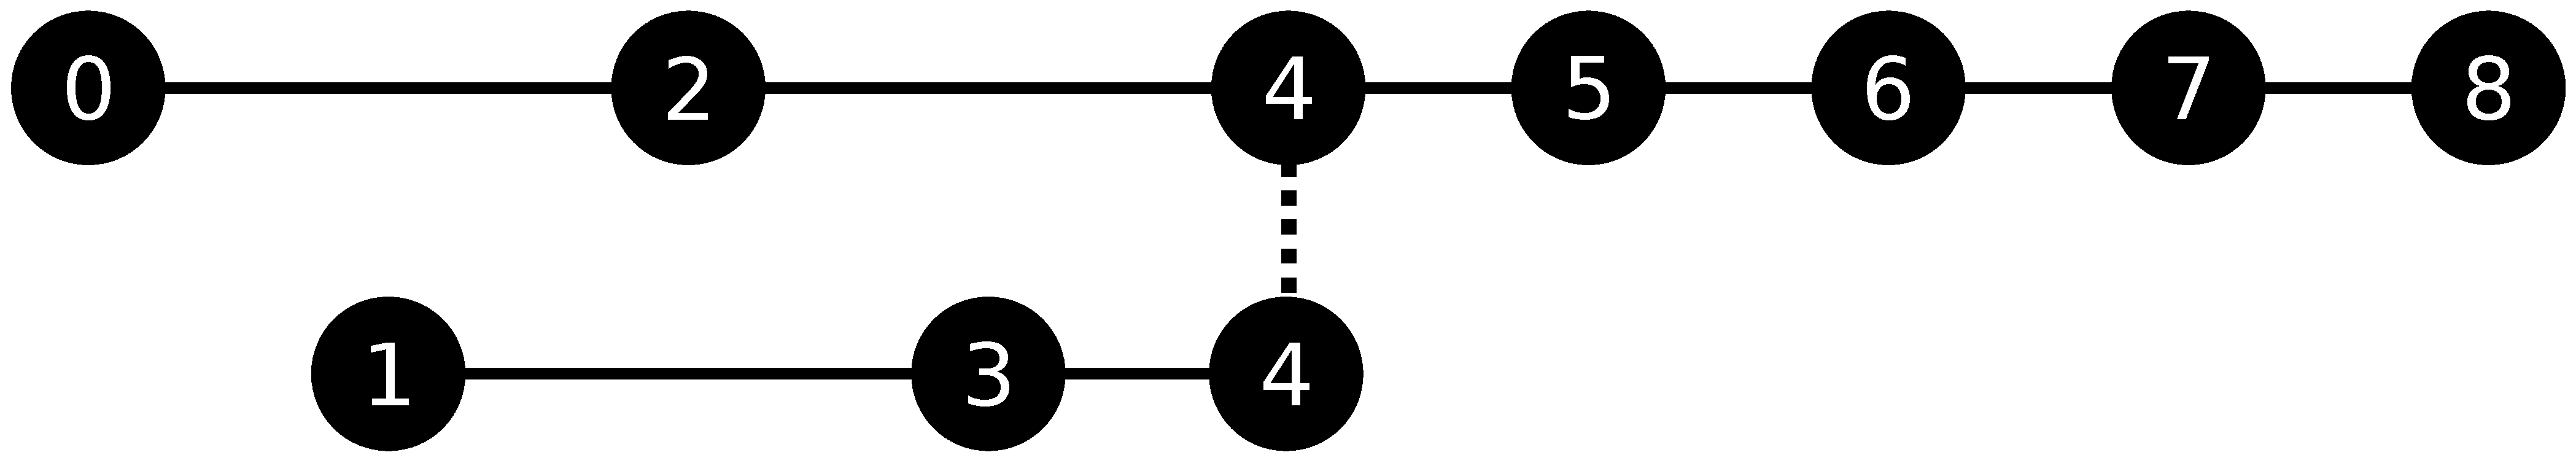
\includegraphics[scale=0.12]{./images/w3x3-split-tree-decomposition.eps}}}%
    \caption{Branch Decomposition of the split tree.}%
    \label{fig:example}%
\end{figure}



\begin{figure}[h]%
    \centering
    \subfloat[$X_1$]{{
\includegraphics[scale=0.05]{./images/filtration/asc/x1.pdf}}}%
    \qquad
    \subfloat[$X_2$]{{
\includegraphics[scale=0.05]{./images/filtration/asc/x2.pdf}}}%
    \qquad
    \subfloat[$X_3$]{{
\includegraphics[scale=0.05]{./images/filtration/asc/x3.pdf}}}%

    \subfloat[$X_4$]{{
\includegraphics[scale=0.05]{./images/filtration/asc/x4.pdf}}}%
    \qquad
    \subfloat[$X_5$]{{
\includegraphics[scale=0.05]{./images/filtration/asc/x5.pdf}}}%
    \qquad
    \subfloat[$X_6$]{{
\includegraphics[scale=0.05]{./images/filtration/asc/x6.pdf}}}%

    \subfloat[$X_7$]{{
\includegraphics[scale=0.05]{./images/filtration/asc/x7.pdf}}}%
    \qquad
    \subfloat[$X_8$]{{
\includegraphics[scale=0.05]{./images/filtration/asc/x8.pdf}}}%
    \qquad
    \subfloat[$X_9$]{{\includegraphics[scale=0.05]{./images/filtration/asc/x9.pdf}}}%

    \caption{Ascending Filtration of the Dataset.}%
    \label{fig:example}%
\end{figure}


\begin{figure}[h]%
    \centering
    \subfloat[$X^9$]{{
\includegraphics[scale=0.05]{./images/filtration/desc/x1.pdf}}}%
    \qquad \qquad
    \subfloat[$X^8$]{{
\includegraphics[scale=0.05]{./images/filtration/desc/x2.pdf}}}%
    \qquad \qquad
    \subfloat[$X^7$]{{
\includegraphics[scale=0.05]{./images/filtration/desc/x3.pdf}}}%

    \subfloat[$X^6$]{{
\includegraphics[scale=0.05]{./images/filtration/desc/x4.pdf}}}%
    \qquad \qquad
    \subfloat[$X^5$]{{
\includegraphics[scale=0.05]{./images/filtration/desc/x5.pdf}}}%
    \qquad \qquad
    \subfloat[$X^4$]{{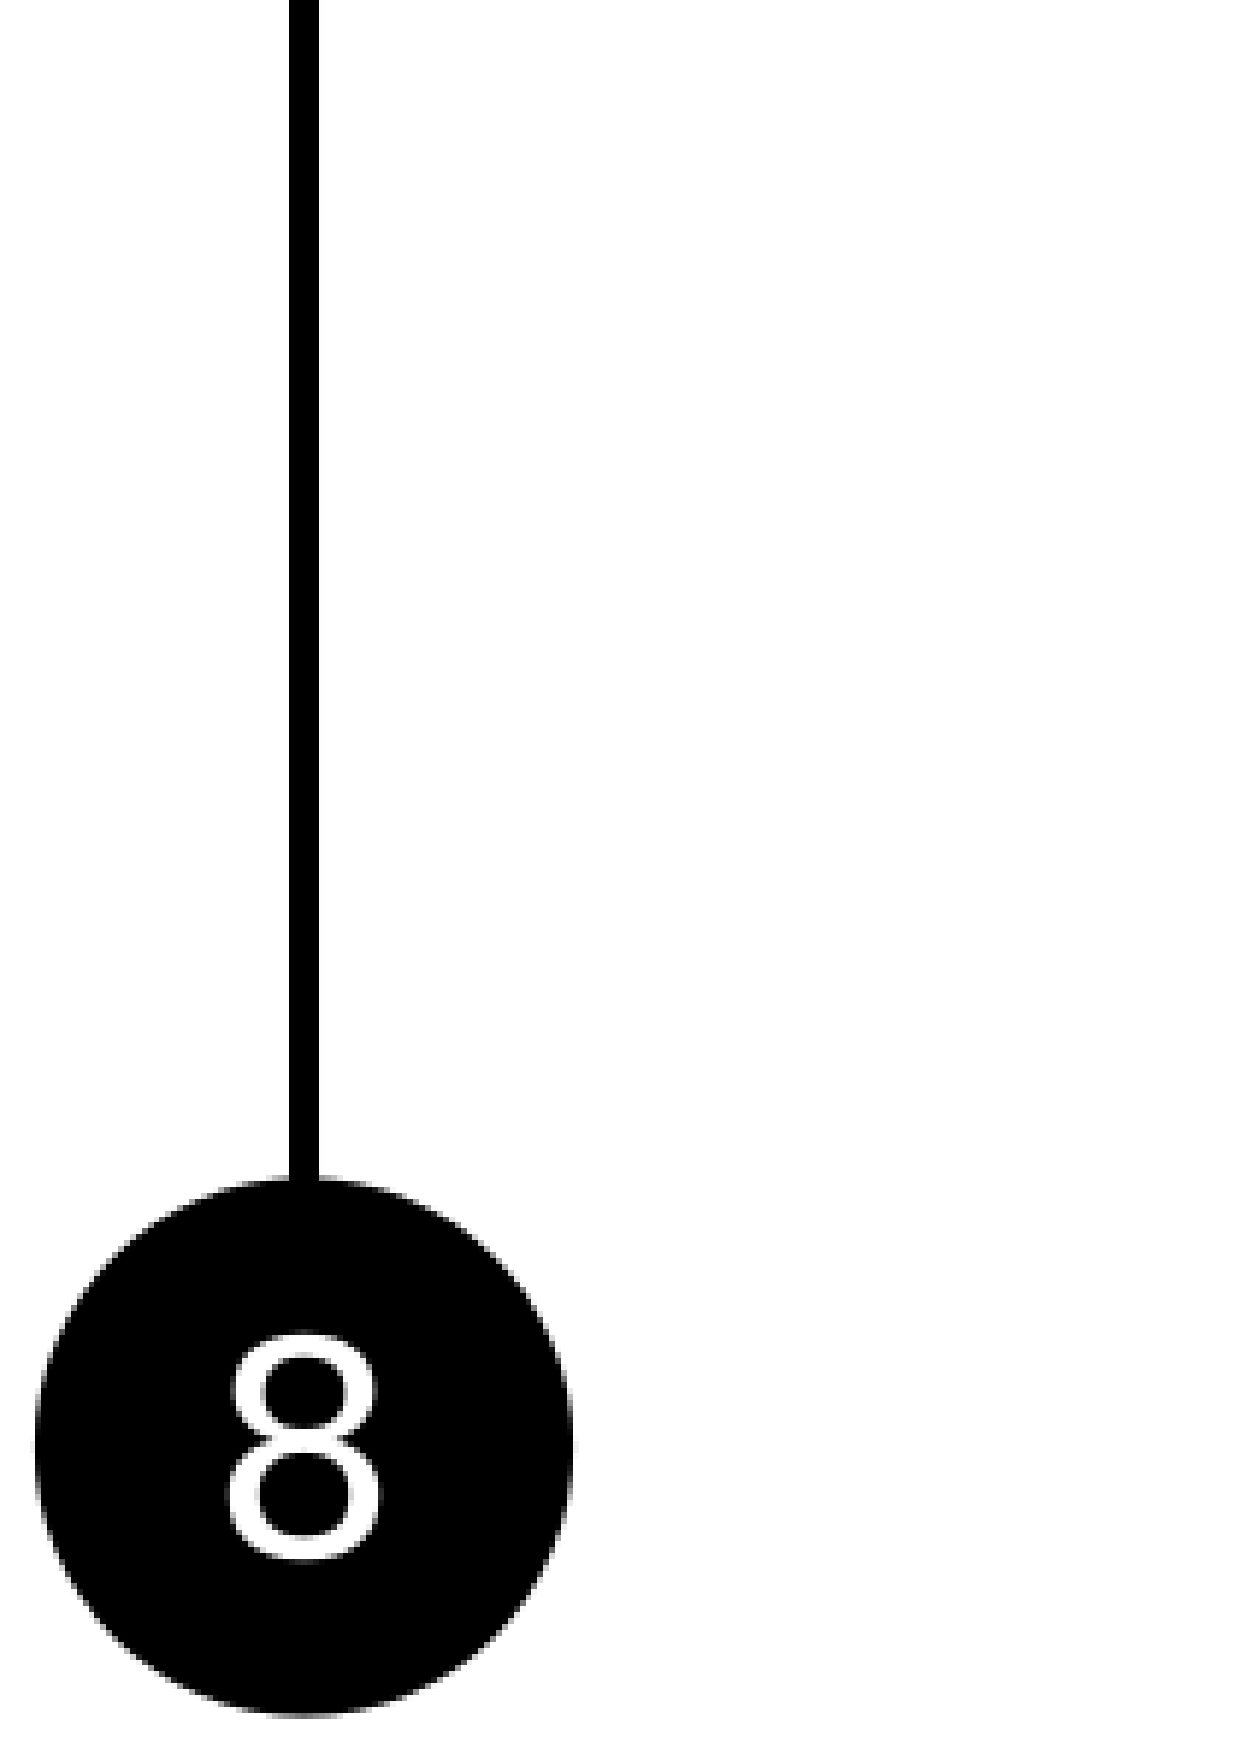
\includegraphics[scale=0.05]{./images/filtration/desc/x6.pdf}}}%

    \subfloat[$X^3$]{{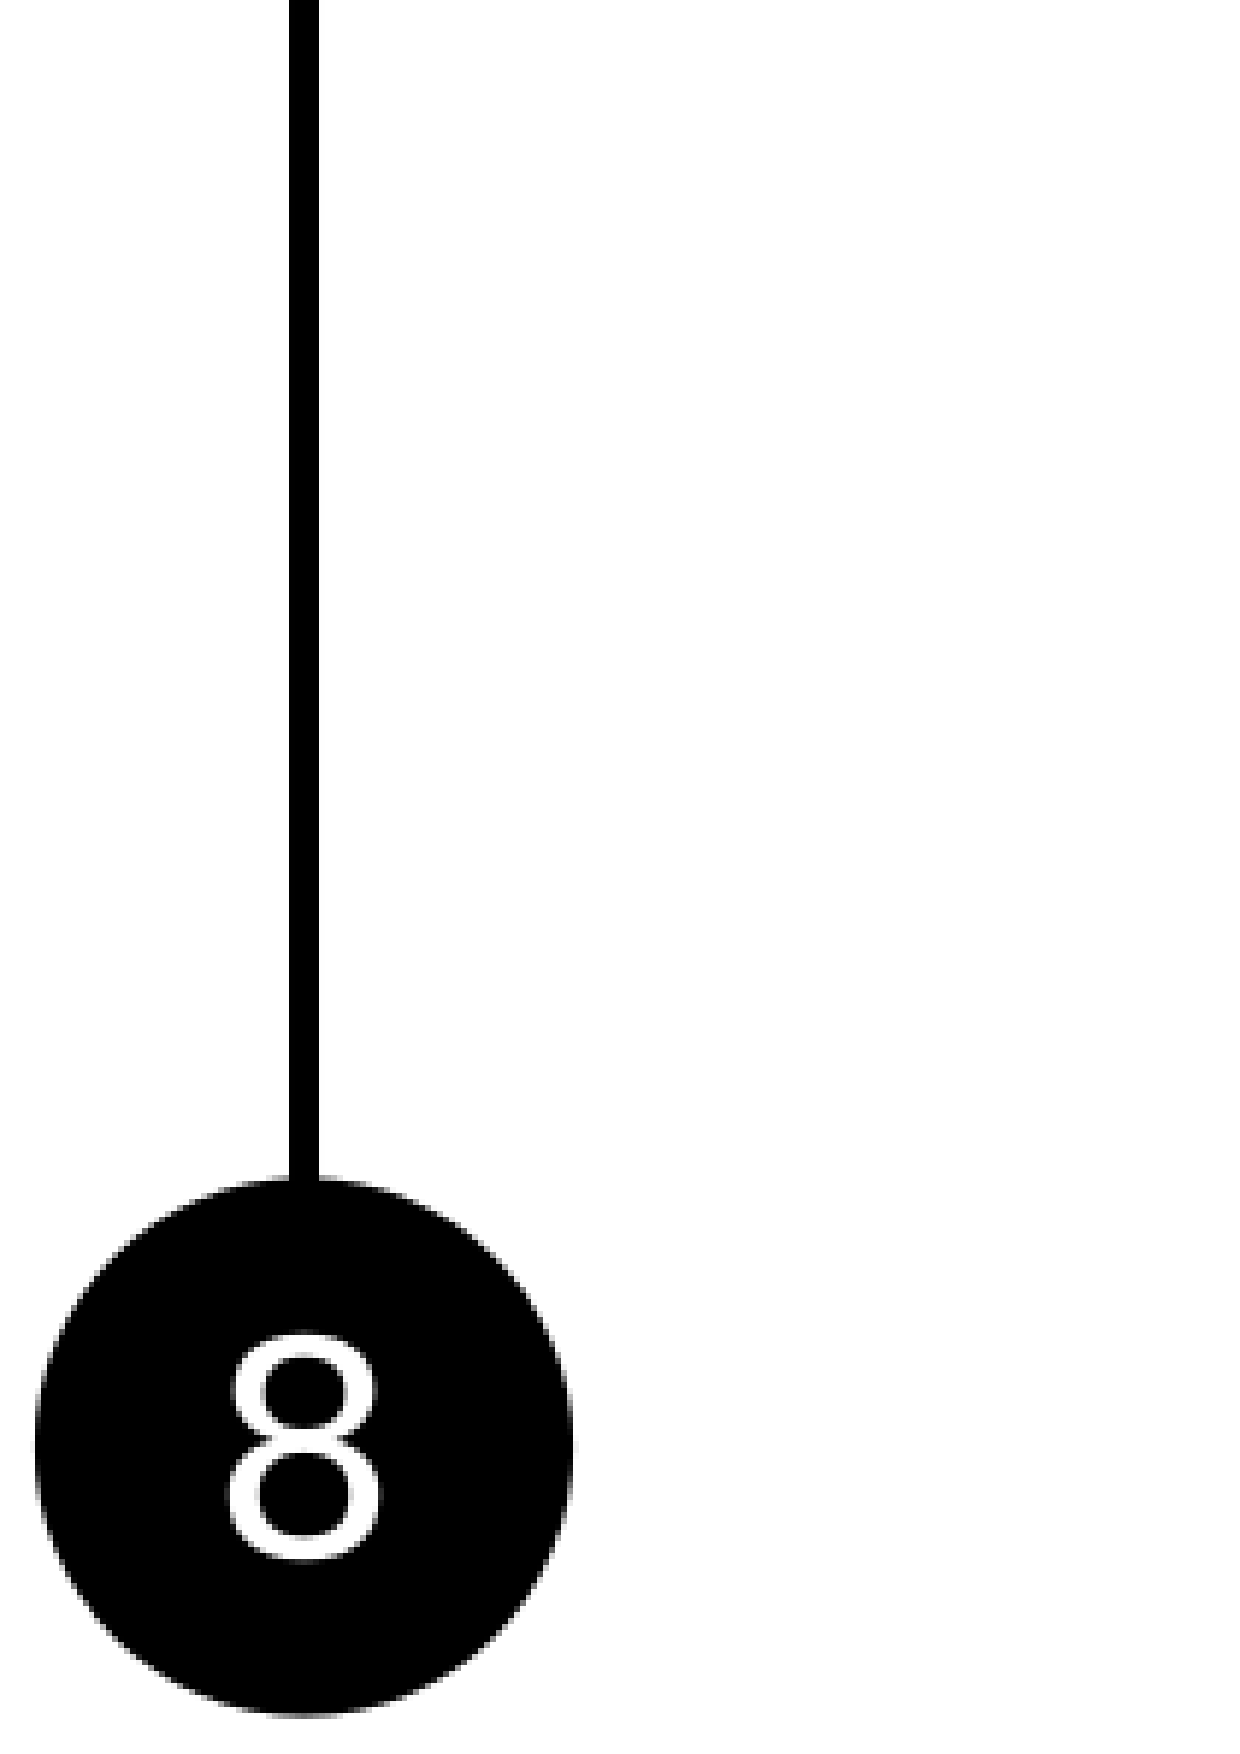
\includegraphics[scale=0.05]{./images/filtration/desc/x7.pdf}}}%
    \qquad \qquad
    \subfloat[$X^2$]{{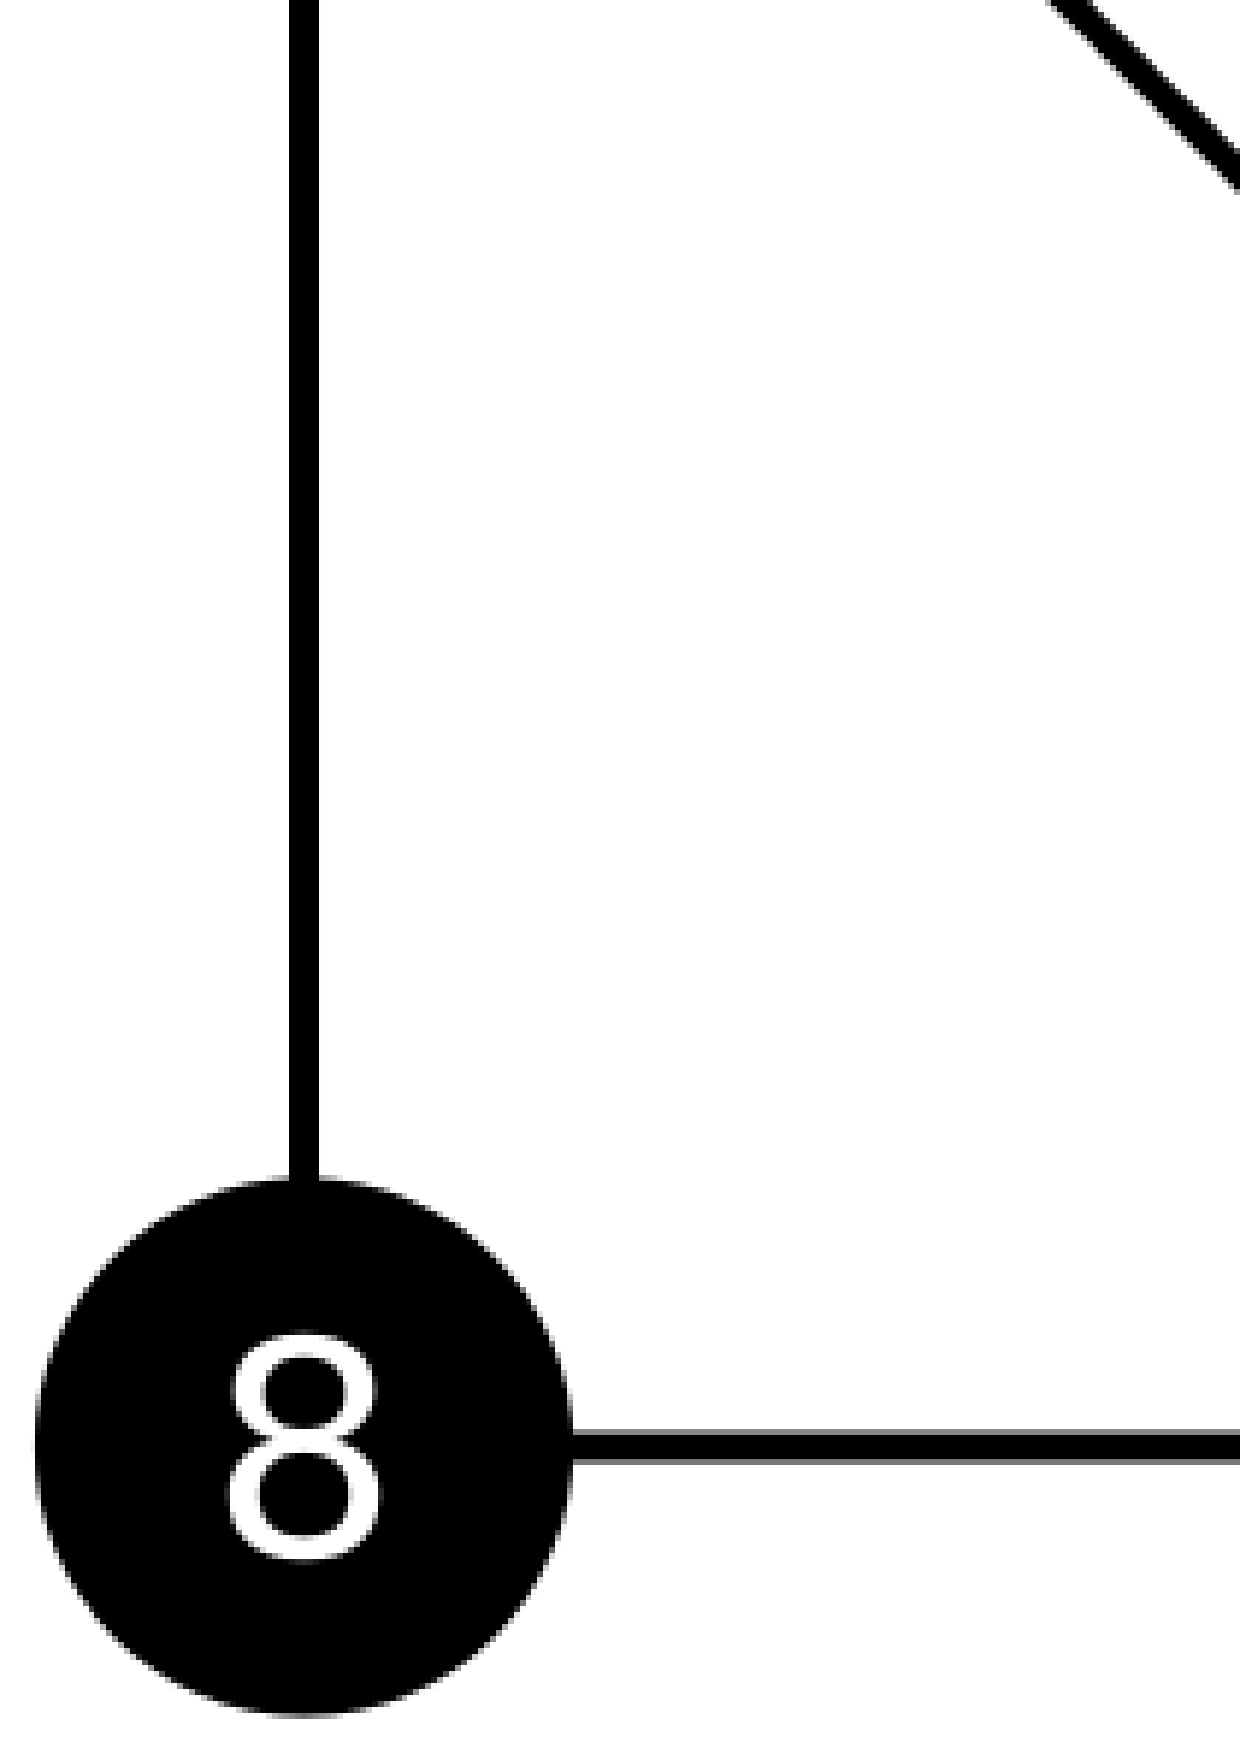
\includegraphics[scale=0.05]{./images/filtration/desc/x8.pdf}}}%
    \qquad \qquad
    \subfloat[$X^1$]{{\includegraphics[scale=0.05]{./images/filtration/desc/x9.pdf}}}%

    \caption{Descending Filtration of the Dataset.}%
    \label{fig:example}%
\end{figure}


\begin{figure}[h]%
    \centering
    \subfloat[Ascending Filtration]{{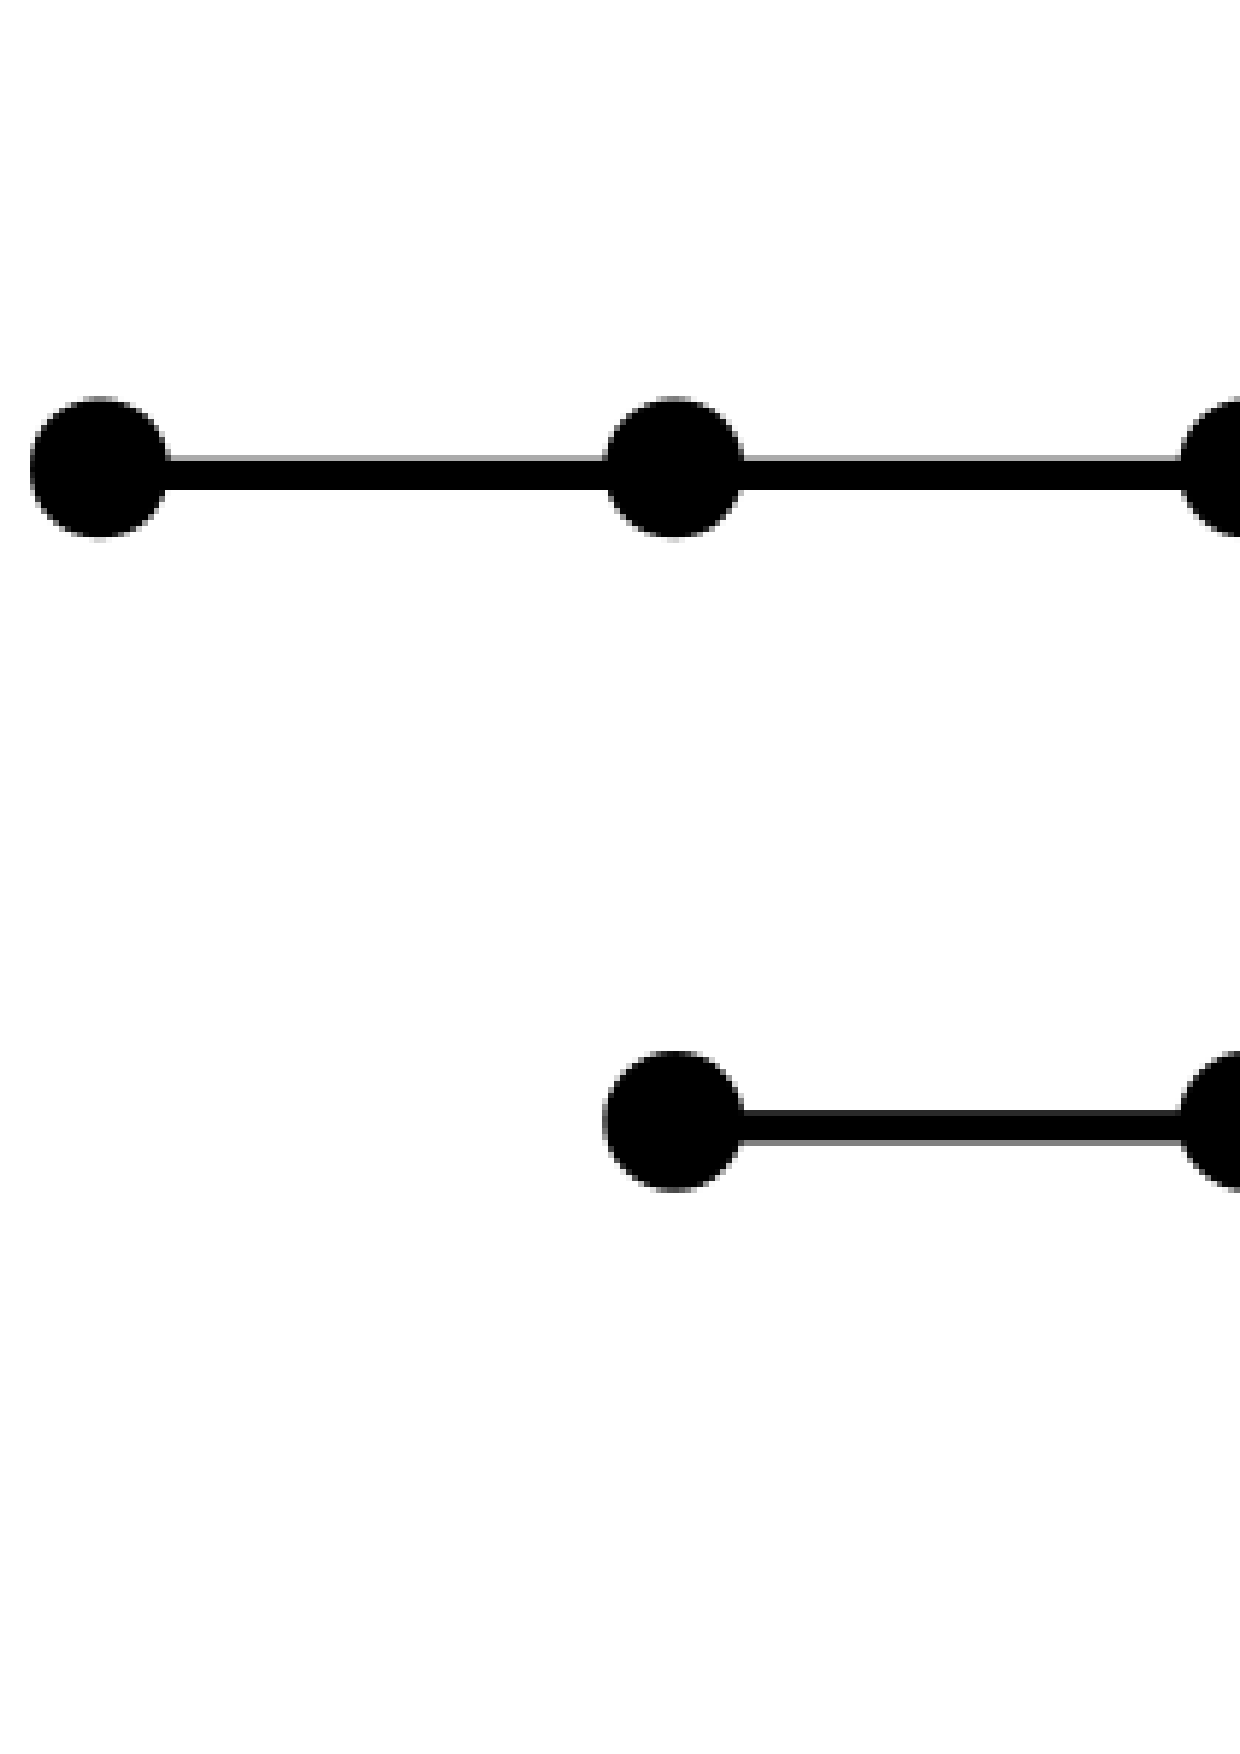
\includegraphics[scale=0.08]{./images/filtration/asc-filtration.pdf}}}%
    \qquad \qquad
    \subfloat[Descending Filtration]{{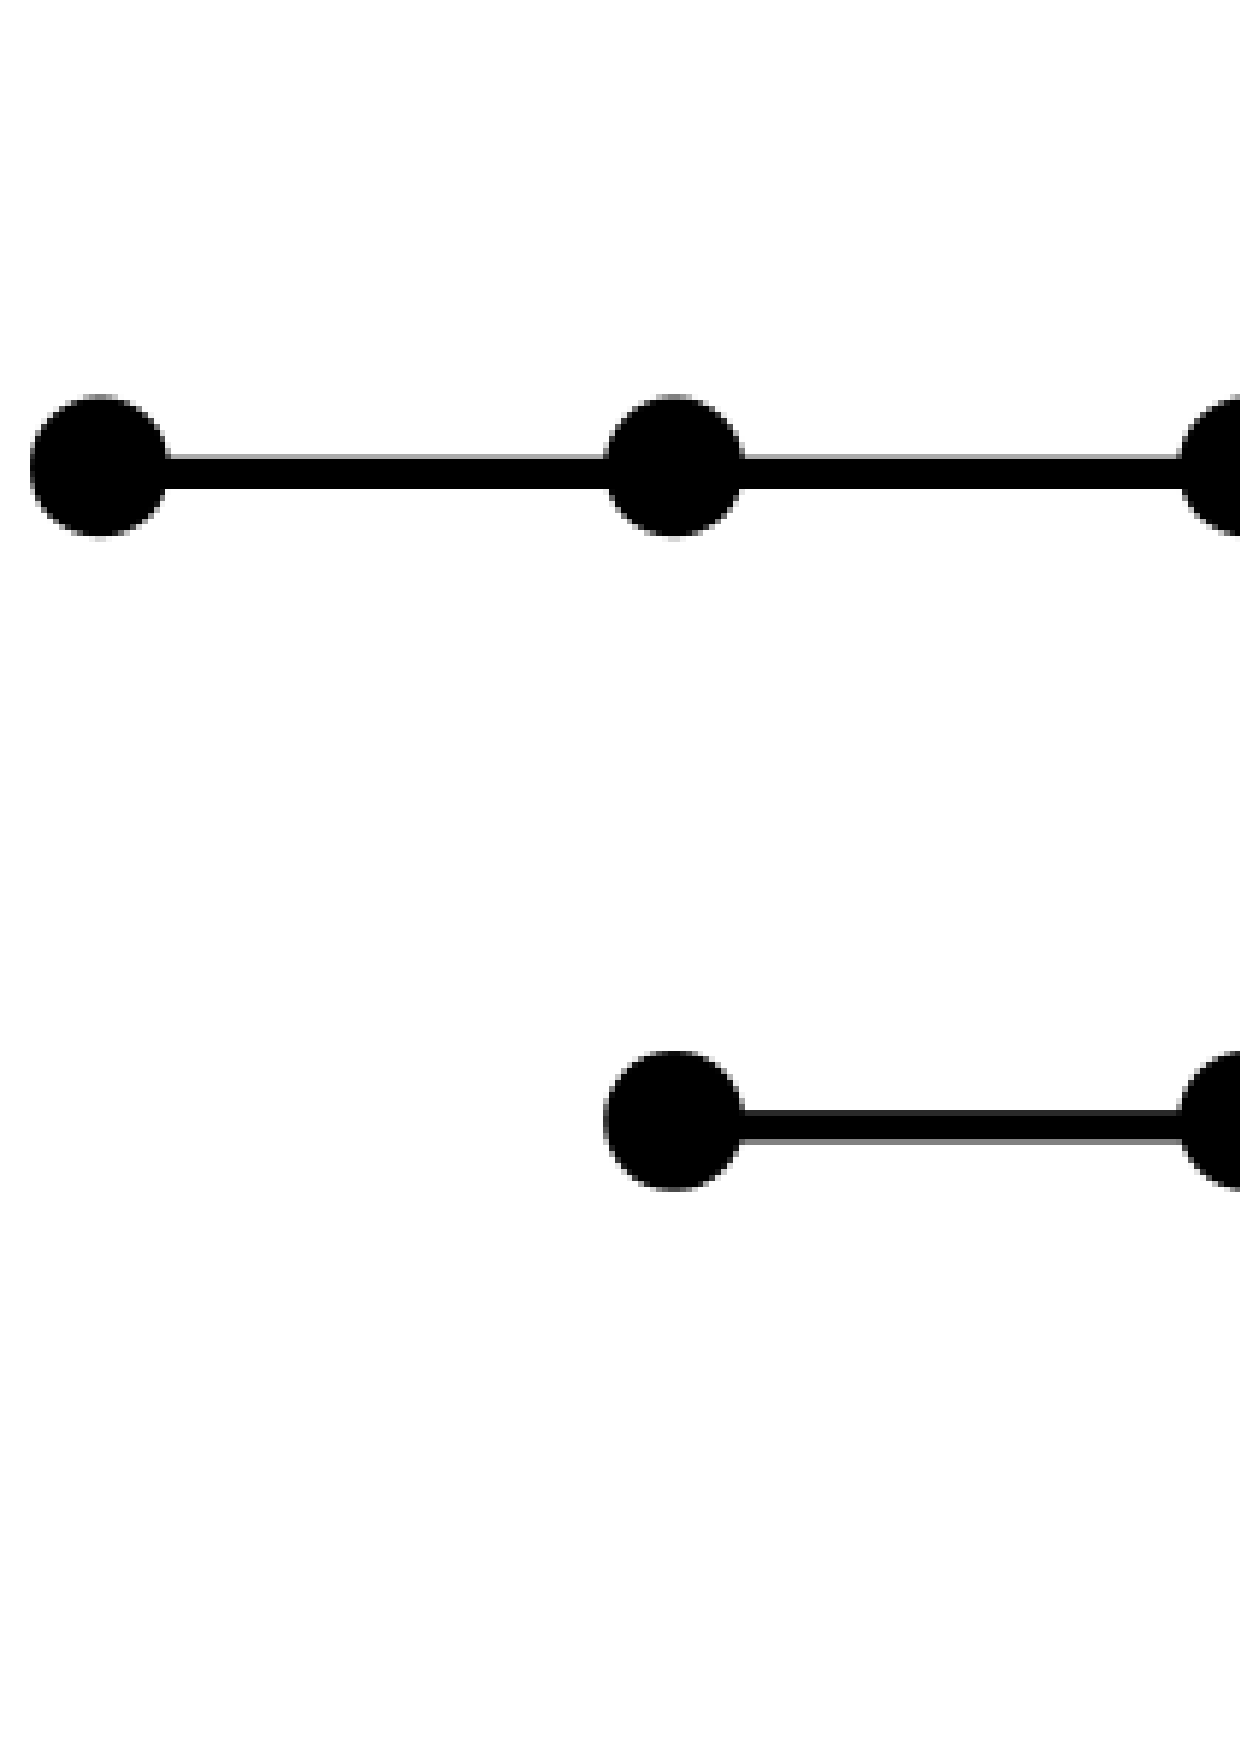
\includegraphics[scale=0.08]{./images/filtration/desc-filtration.pdf}}}%

    \caption{Barcode Diagrams of the Persistent Homology of the ascending and descending filtration.}%
    \label{fig:example}%
\end{figure}

% What we have uncovered is not the complete story. There is a deeper connection between extended persistence and contour trees in general. If we look at alternative algorithms for constructing the 0th homology specifically we can see that the extended persistence of an ascending filtration is equivalent to branch decomposition of the join tree and the extended persistence is equivalent to a branch decomposition of the split tree.

% Going back to the claim made \cite{ct-branch-decomp} we see that there is truth to it if we adjust it to extended persistence and apply specifically to join and split trees. Here future questions that arise based on this fact.

% \begin{itemize}
%     \item By using the persistence pairs on other homology group we can produce split and join tree for the cycles, void, etc... We can them combine them like we combine the join and split trees for the contour. What kind of a structure does that yield?
%     \item Can we compute the contour tree directly from homology. Can we find a natural continuous function between the level sets of a filtration. Would the persistence of this sequence be equivalent to the contour tree. In higher dimensions would be equivalent to the previous point?
%     \item Who killed Laura Palmer and will the new Twin Peaks be good?
% \end{itemize}



%In this final section we will present examples for how extended persistence on the 0th homology is actually equivalent to computing join and split tree.

%*Don't know if I can prove this yet, but it probably won't be too hard. But then again it may be.*

%*Should I keep this or not?*







% @TODO Check spelling in references.



%Let us now restrict $M$ to be compact and contractable. This will ensure that the Reeb Graph of $M$ is a Contour Tree. We would like to tackle the claim made in \cite{ct-branch-decomp} that the persistent homology pairs are equivalent to branch decomposition pairs. We can immediately see that this claim is either false of ill-defined. The major reason for this is that essential homology classes do not get paired. But in the branch decomposition schemes all critical points are paired.

%There is however yet more reason to pursue this. Slightly after the paper of branch decomposition was published, there emerged a way to extend the persistent homology scheme so that all critical points get paired. Using this will allows us to directly compare it to the branch decomposition of a contour tree.




%Lastly we will not that we cannot take into account the



%Explain the claim that has been made and quote it directly.

%Show why it is flawed in the first place.

%Show why it's not equivalent to it.



%* Most of this sections will be pictures this is why it is not written up properly *

%Now let us examine the relation of extended persistence to branch decomposition. Here is an example branch decomposition of a contour tree of the following 3x3 grid dataset. It is not possible for the branch decomposition to pair the global maximum with the global minimum. There is no monotone path between them. To show that no branch decomposition of a contour tree is equivalent to the extended persistence of the dataset I will demonstrate that extended persistence necessarily pair the global minimum with the global maximum.

%*Show the extended persistence filtration of the W3x3*
%*Show the branch decomposition*


% @TODO Add quote
%As you can see these methods produce very different pairings. We will conclude that the claims made in [] are either false of not well defined. The correct way to phrase this is the following. "Our definition of persistence is quivalent to extended persistence for the join and split trees. It is not directly applicable in the case of the contour tree itself in terms of the formalism it's built on".


%It so happens that a w-structure that this dissertation is devoted to causes not only computational difficulties, but also serve as counterexamples to pose theoretical difficulties as well. To further cement statement we will us show a more general general result in the following chapter which holds for all filtrations of path-connected spaces.


%The maps in the ascending filtrations are induced via the inclusion maps between the nested spaces $M_i \subseteq M_j$  where $i \le j$. The more interesting case if between the relative homology groups. First of all the isomorphism between $H_n(M) = H_n(M, M^{c_n})$ comes from that fact that $M^{c_n} = \emptyset$ and quotienting by the empty sets leaves a group unchanged. The show where the consecutive maps come from we will give the following example.

%Let $X$ be a simplical complex, $B \subset X$ be a subcomplex of $X$ and $A \subset B$ be a subcomplex of $B$. Then we can find a natural map from $H_n(X, A)$ to $H_n(X, B)$ induced by the inclusion from $A$ to $B$. Let us write out $C_n(X), C_n(A), C_n(B)$ through their generator simplicies.

% @TODO Fix these brackets
%$$ C_n(X) = <a_1, a_2, ..., a_k, ..., a_l, ..., a_n> $$
%$$ C_n(A) = <a_l, ..., a_n>$$
%$$ C_n(B) = <a_k, ..., a_l, ..., a_n>$$


%Then the relative chains are generated by:

%$$ C_n(X, A) = <a_1, ..., a_k, ..., a_{l-1}>$$
%$$ C_n(X, B) = <a_1, ..., a_{k-1}>$$


% @TODO Show it is a chain map

%Where we can introduce a natural inclusion map $f : C_n(X, A) \to C_n(X, B)$ where $f(a_i) = a_i$ when $i < k$ and $f(a_i) = 0$ when $i \ge k$. The map $f$ is well defined as an inclusion map and furthermore it is a chain map. Chain maps induce linear maps on the homology. Therefore we obtain the map $f_* : H_n(X, A) \to H_n(X, B)$ where $f_*([\alpha]) = [f(\alpha)]$. Where the brackets denote the homology quotient classes in $H_n(X, A) \text{ and } H_n(X, B)$ respectively.

%Now let us to back to the descending filtration of $M$. We have

%Let us go back extended persistence. In the descending filtration of the relative homology we have the scenario we just described. Therefore as there is an inclusion function for between every $M^{c_i}$ and every $M^{c_j}$ where $i \ge j$ and this induces a linear map between every $H_n(M, M^{c_i})$ and $H_n(M, M^{c_j})$.

%We have developed all this mathematical machinery

%-- Give some intuition behind this.

%-- Show how this is used on an example.

%-- Give an algorithm for computing it.

%-- Explain how the algorithm is connected to the computation.

%\section{Persistent Homology and the Contour Tree}

%-- Say some general things about how we are going to relate the two and what we shall accomplish in this chapter.

%\subsection{Join and Split Trees}

%Show that the computation of the ascending filtration and descending filtration is equivalent to the join and split tree of a contractable domain.

%Show the it is equivalent to branch decomposition of the join and split tree.

%Show that extended persistence pairing are not equivalent to branch decomposition pairing. Say the paper is either wrong or had something else in mind which is not clarified well enough.

%Emerge victorious and have the plebeians chant you name in the streets. All Hail Petros all hail Petros.



% In order to produce a detailed computation of the persistent homology of a filtration we would have to compute all homology groups of all complexes and then compute all inclusion maps. Doing so by hand is cumbersome and more importantly far too lengthy. We will avoid doing it in favour of presented diagrams of the evolution of the homology classes and appeal to the reader's geometric and topological intuition to argue their correctness.

% *Let us look at the following example. Show a pretty picture and explain it*

% @TODO Why is this true?
% There is a theorem that states that the persistence digram of a filtration encodes all of the information about the persistent homology groups.
%
% *Examples*

% Finally we will describe an algorithm for computing the persistence pairs. It requires us order all of the simplices in the complex $\sigma_1, \sigma_2, ..., \sigma_n$ according to these rules \cite{ph-a-survey}.
%
% \begin{itemize}
%     \item $\sigma_i$ precedes $\sigma_j$ when $\sigma_j$ was introduced later in the filtration than $\sigma_i$
%     \item $\sigma_i$ precedes $\sigma_j$ when $\sigma_i$ is a face of $\sigma_j$
% \end{itemize}
%
% Not instead of having to compute the homology groups of all complexes in the filtration individually and then computing the induces maps we can perform the whole computation in a single matrix reduction. Let $D$ be an $n\times n$ matrix and such that.
%
%    $$
%    D[i, j] = \left\{
%        \begin{array}{@{}l@{\thinspace}l}
%            \text{1}  &: \text{if } \sigma_i \text{ is a codimension 1 face of } \sigma_j \\
%            \text{0}  &: \text{otherwise} \\
%        \end{array}
%    \right.
%    $$
%
% In other matrix $D$ is a matrix that holds the boundaries of all simplicies in a single matrix. It is called the combined boundary matrix. Now we can perform the following reduction just by column operations.
%
%
% \begin{algorithm}
% \caption{Reduce Combined Boundary Matrix}
%
% \begin{algorithmic}[1]
%
%
% \ForAll {j $\in$ \{1, 2, ..., n\}}
%     \While {$\exists j': j' < j \text{ and } low(j') == low(j) $}
%         \State Add column $j'$ to column $j$.
%     \EndWhile
% \EndFor
%
% \end{algorithmic}
% \end{algorithm}
%
% The proof of this algorithm is outlined in \cite{persistence-original}.

%
% Finally we will define what we call the persistence of a homology class.
%
% \begin{defn} The persistence of a single homology class in persistent homology that is born at time $t_1$ and dies at time $t_2$ is $t_1 - t_2$.  \end{defn}
%
% % @TODO Do this
%     There are two primary ways to visualize the persistence pairing produces by persistent homology. The first in through persistence diagrams \cite{comp-topo}. In the persistence diagrams the pairs are visualised as points in the Carthesian coordinate system above the main diagonal $y = x$. Example []. The second way is through barcode diagrams. You can see the barcode digram on fig[]. For every simplical complex in the filtration we have a number of starting lines equal to the number of generators for the homology classes. These lines feed into each other according to where the induced by inclusion homomorphism take them in the next simplical complex.
%
%
% % @TODO Return these.
%
% %\begin{figure}[h]%
%     %\centering
%     %%\includegraphics[scale=0.085]{./images/chapter4/bar-diagram.eps}%
%     %\caption{Barcode Diagram of a Filtration}%
%     %\label{fig:bar-diag}%
% %\end{figure}
%
% %\begin{figure}[h]%
%     %\centering
%     %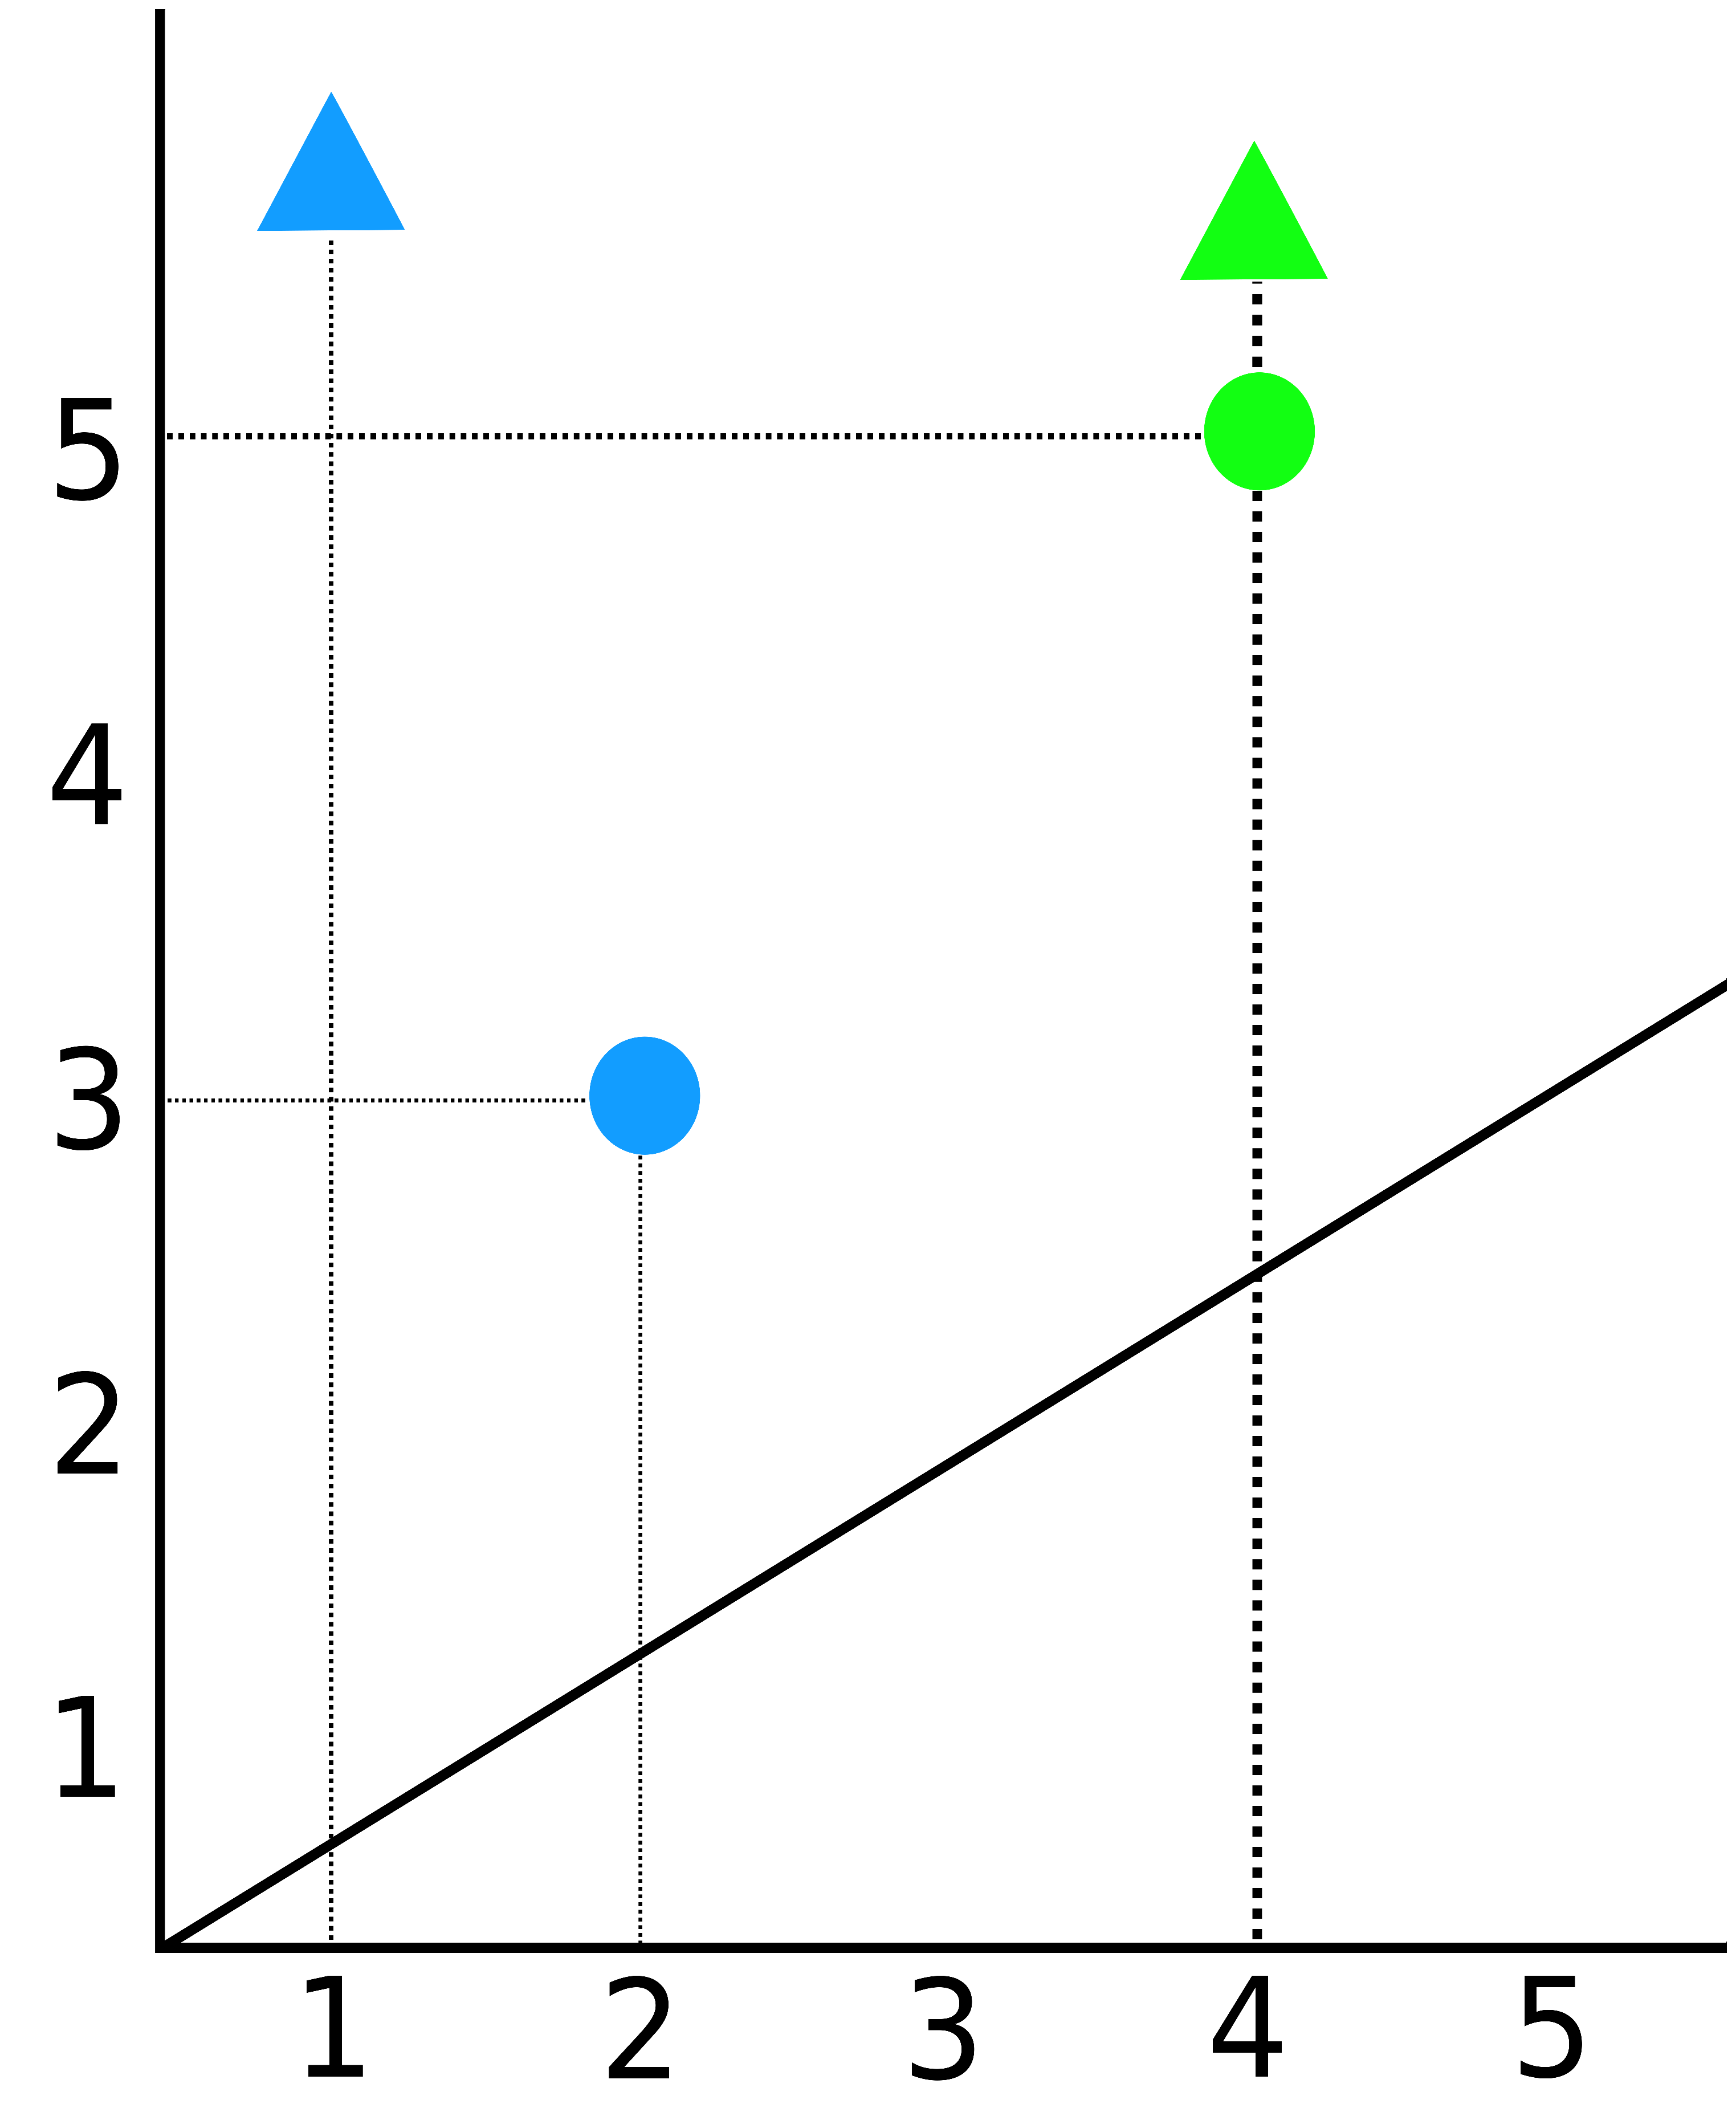
\includegraphics[scale=0.085]{./images/chapter4/diagram.eps}%
%     %\caption{Persistence Diagram of a Filtration}%
%     %\label{fig:per-diag}%
% %\end{figure}
%
%
% % @TODO Add reference
% % Furthermore when two classes merge we must choose which one survives and which one dies. By established convention [] we will use the Elder Rule. By the Elder Rule the class that was born first continues to persistent and the younger one is destroyed.
%
%
% %Here are two examples of filtrations and explanations of bar diagrams.
%
%
% %Let us now restrict $M$ to be compact and contractable. This will ensure that the Reeb Graph of $M$ is a Contour Tree. We would like to tackle the claim made in \cite{ct-branch-decomp} that the persistent homology pairs are equivalent to branch decomposition pairs. We can immediately see that this claim is either false of ill-defined. The major reason for this is that essential homology classes do not get paired. But in the branch decomposition schemes all critical points are paired.
%
% %There is however yet more reason to pursue this. Slightly after the paper of branch decomposition was published, there emerged a way to extend the persistent homology scheme so that all critical points get paired. Using this will allows us to directly compare it to the branch decomposition of a contour tree.
%
% %We will now show that computing the persistent homology of the descending and ascending filtration of $M$ is equivalent to constructing the join and split tree of $M$ respectively.
%
% %* Show that this is the case *
%
% %* SHOW EXAMPLES *
%
% % Define extended persistence.


% A natural thing to do would be to directly apply persistent homology twice. Once on the ascending and the on the descending filtration. The problem that arises is in relating the classes of the two filtrations. We cannot merge both filtrations into a single long chain because the induced maps of the two filtrations flow in different directions :
%
% $$ 0 = H_n(M_{c_1}) \rightarrow ... \rightarrow H_n(M_{c_n}) = H_n(M) = H_n(M^{c_1}) \leftarrow ... \leftarrow H_n(M^{c_{n}}) = 0.$$
%
% The direction of the arrows is accordance with the how the homomorphisms are induced. To verify this consider that $M_{c_i} \subseteq M_{c_j}$ and $M^{c_j} \supseteq M^{c_j}$ for $i \le j$. What we would like to achieve it to reach $H_n(M)$ in the ascending filtration and to start a new filtration which reduces it to the zero group by "removing" simplicies from it. We cannot do so in absolute homology because we would not have inclusion maps. We can however achieve this with relative homology. Consider the filtration:
%
% $$ H_n(M) = H_n(M, M^{c_n}) \rightarrow H_n(M, M^{c_{n - 1}}) \rightarrow ... \rightarrow H_n(M, M^{c_{1}}) = 0 $$


% @TODO By which def (end of paragraph)
% In this relative filtration the linear maps are induced by inclusions on the relative homology groups. To see this let $(M, M^{c_i})$ and $(M, M^{c_{i+1}})$ two consecutive pairs. The inclusion map from $M$ to $M$ takes the superlevel set $M^{c_i}$ in the superlevel set $M^{c_{i+1}}$ because $M^{c_i} \subseteq M^{c_{i+1}}$. By definition [] this is a simplicial map from $(M, M^{c_i})$ and $(M, M^{c_{i+1}})$ and thus induces a homomorphism between $H_n(M, M^{c_i})$ and $H_n(M, M^{c_{i+1}})$.

% The final step to complete our desired sequence is to "glue" these two filtrations together at the point $ H_n(M_{c_n}) = H_n(M) = H_n(M, M^{c_n})$. The second equality holds because $M^{c_n} = \emptyset$ and quotienting by the empty set leaves the underlying relative chain complexes unchanged. Putting this all together yields the following chain of homology groups.
%
% $$ 0 = H_n(M_{c_1}) \rightarrow ... \rightarrow H_n(M_{c_n}) = H_n(M) = H_n(M, M^{c_n}) \rightarrow ... \rightarrow H_n(M, M^{c_{1}}) = 0.$$
%
% % @TODO Is that really what a close subcomplex is?
%
% This augmented filtration justifies the pairing of essential classes according to the intuitive understanding we obtained from example []. The only issue is that the relative homology groups are difficult to interpret on their own. To aid our comprehension of what exactly occurs in the relative filtration we shall employ the Excision Theorem where $H_n(M, M^{c_i}) = H_0(M / M^{c_i}, pt) = \overset{\sim}{H}_0(M / M^{c_i})$ where $M^{c_i}$ is a closed subcomplex of $M$ as required for all $i \in \{1, 2, 3, ..., n\}$.
%
% * Take a look at example how the complex is built and the how it unwinds itself *
%
% 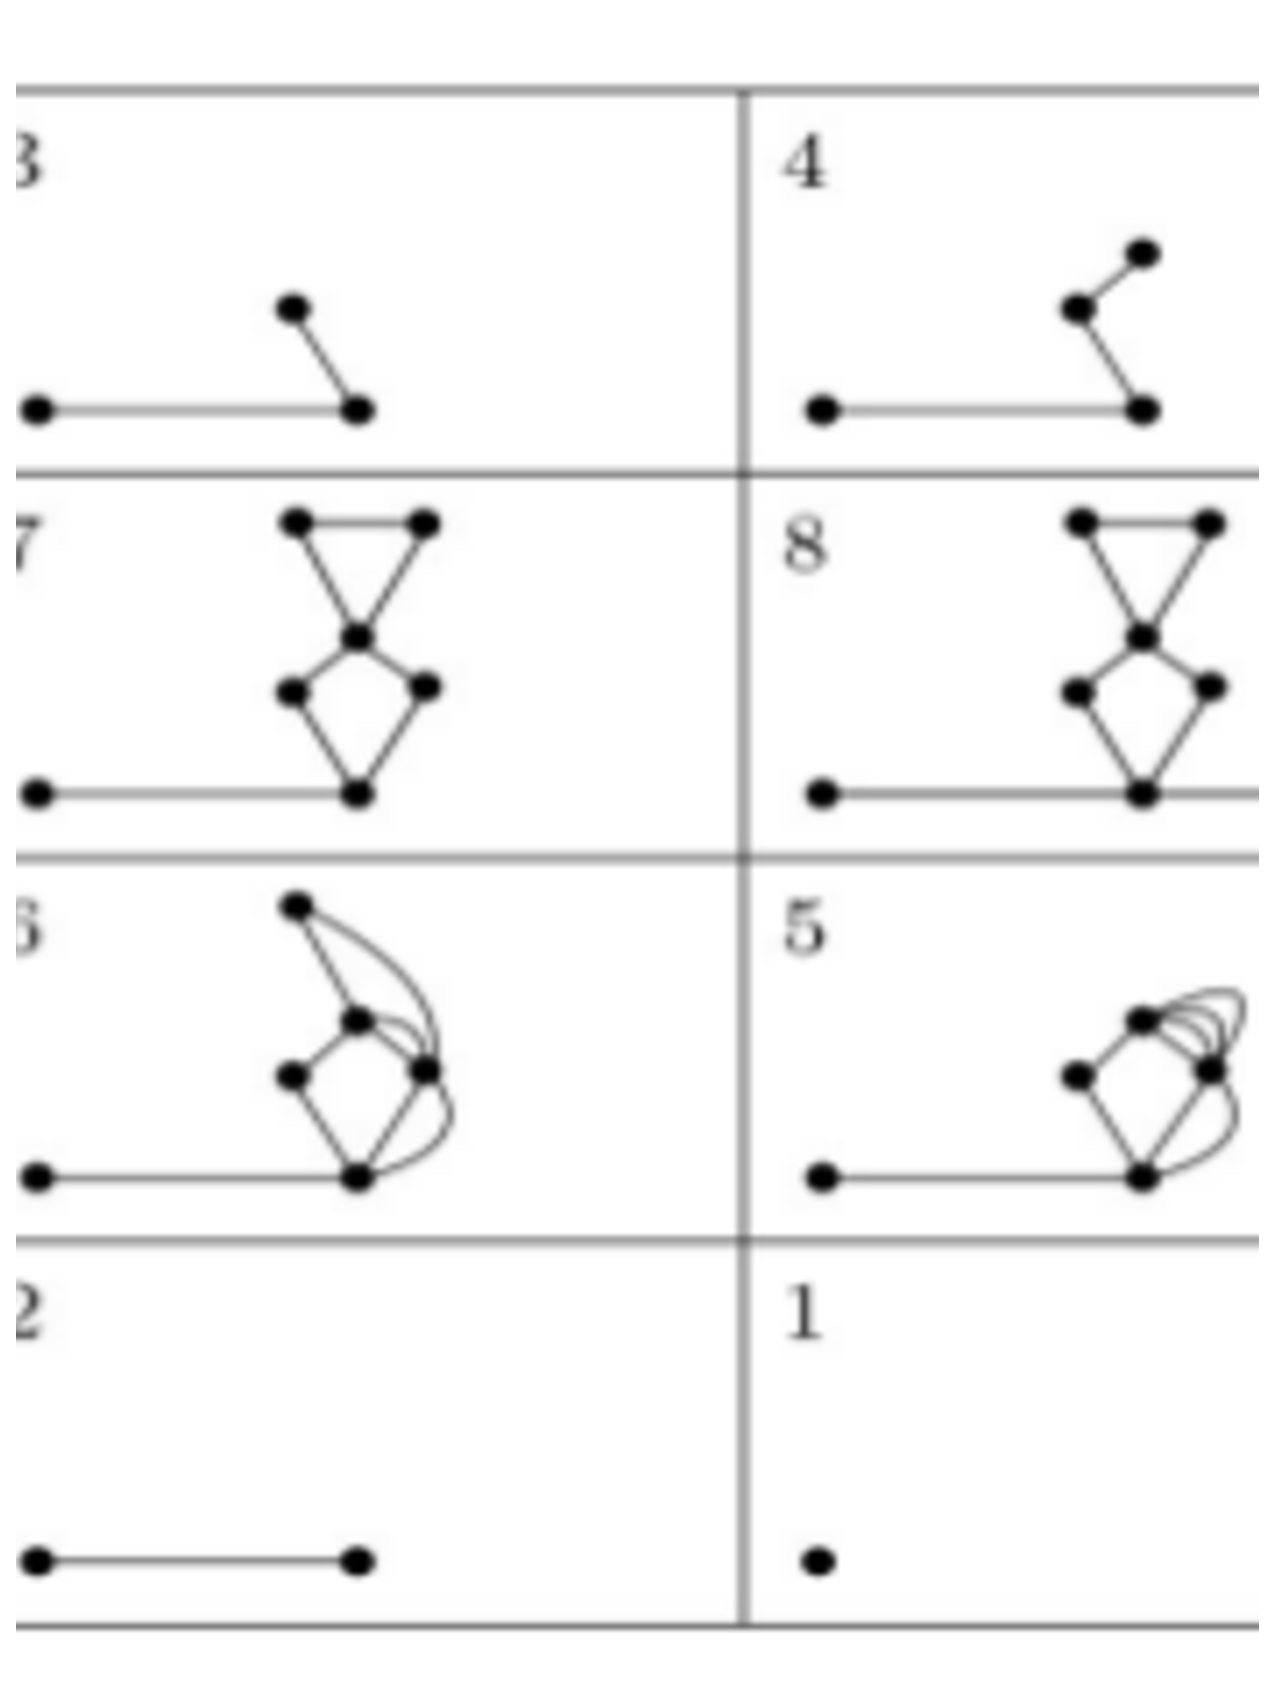
\includegraphics[scale=0.2,center]{./images/extended-ph.eps}


% Let us unpack the claim piece by piece. Firstly the paper only redefines how the persistence of the branches is computed and branches are pair of critical points. Therefore for this to be equivalent to the persistence pairs, both methods must  produce equivalent pairs. It is clear from this definition that the actual persistence pairings stay the same, we only compute the persistence value in a different way. What we will aim to show is that the pairings produced by persistent homology are in themselves different from the pairings produces by branch decomposition. After this it will not matter how the actual persistence of branches is computed as they are fundamentally different things. Lastly the paper claims that the branch decomposition definition differs from persistent homology in that "it takes into consideration the topological obstructions.". It is not clear exactly what the authors meant by "topological obstructions". These obstructions are not defined in the paper nor in subsequent publications. This does not stop us from working with the definition because we will demonstrate a second way in which persistence differs from branch decomposition.

% The first major difference we can find comes from the fact that persistent homology as it was originally defined does not pair all critical points. As we discussed previously the pairings of essential homology classes are not defined because they never die in the filtration. In the case of contour trees we will be dealing will simply connected contractable domains. Such domains have a single connected component and therefore have exactly one essential homology class in the 0th homology. This is the class that is born at the global minimum, or the first simlicial complex in the filtration. In branch decomposition on the other hand all critical points are paired.

% This is already of major difference between the two. Furthermore the paper on branch decomposition clearly cites the original paper for persistent homology and not the subsequence paper on extended persistence where this issue is remedied. In fact it cannot reference that paper. The branch decomposition paper has been published in January of 2004 and the paper that clearly defines Extended Persistence as such has been published in January of 2009 \cite{persistence-extended}. There is however more to this story. The concept of pairing critical points unpaired by persistence goes further back than the 2009 paper and can be traced to the paper \cite{extreme-elevation} which was also published in January of 2004. The paper outlines the initial concept of extended persistence in the specific case of 2-manifolds embedded in $\mathbb{R}^3$. This means that the idea of pairing all critical points was present when the claim was made. All of lets us the take this a step further. We will now test whether branch decomposition is equivalent to extended persistence.

% We will demonstrate that they are not with a small counter example. This counter example will show that at least one pair in both is necessarily different. In contour trees where the global minimum and the global maximum are not connected via a monotone path branch decomposition cannot by definition pair them as the endpoints of a branch. Extended persistence on the other hand does pair them as the global maximum is the first class in the descending relative filtration that is homologous to the essential class born at the global minimum. To reduce the stress caused by the reader's feverish anticipation of this counter example we will foreshadow that it is a contour tree with a w-structure. This w-structure is what separates the global minimum from the global maximum.

%
% \subsection{Extended Persistence on Path-Connected Domains}
%
% The final step we take on this journey will be to prove the following original and more general result.
%
% \begin{prop} In the extended persistence of filtration a Morse function with a Path-Connected domain the global minimum pairs with the global maximum in the 0th homology \end{prop}
%
% \begin{proof}
%     Let $M$ be a Path-Connected domain and let $M_1 \subseteq M_2 \subseteq ... \subseteq M_n$ be a filtration of $M$. This filtration induces etended persistence
%
% $$ 0 = H_0(M_{c_1}) \rightarrow ... \rightarrow H_0(M_{c_n}) = H_0(M) = H_0(M, M^{c_n}) \rightarrow ... \rightarrow H_0(M, M^{c_{1}}) = 0.$$
%
% As $M$ is Path-Connected it has one path-connected component and therefore $H_0(M) = H_0(M_0) \simeq  \mathbb{Z}_2$.  Our aim here will be to show that all of the $H_0(M, M^{c_i})$ are trivial. This will mean that the single homology class that exists in $H_0(M)$ will die at $H_0(M, M^{c_n})$ which is exactly the global maximum.
%
%
% % @TODO Define Excision
% % @TODO  Add the thing where this holds - H_n(M / M^{c_i}, pt) = \overset{\sim}{H}_n(M / M^{c_i})
% As a corollary of the Excision Theorem we have that
%
% $$H_0(M, M^{c_i}) = H_0(M / M^{c_i}, pt) = \overset{\sim}{H}_0(M / M^{c_i})$$
%
% where $pt = M^{c_i} / M^{c_i}$.
%
% Now let us explore the reduced homology of the topological space $M / M^{c_i}$. We will show that is it path-connected and therefore the reduced homology is trivial.
%
%
% % @TODO Add quote
% By definition $M$ is path connected. Consider the function $\pi: M \to M/ M^{c_i}$ that takes a point to it's equivalent class. By point set topology [] we know that $\pi$ is continuous. We can also infer that $\pi$ is surjective. Indeed there there is no equivalence class that no point maps to. Furthermore the continuous image of a path connected is connected by []. As we have that $M$ is path-connected therefore $\pi(M) = M / M^{c_i}$ is path-connected.
%
% By [] we have that $H_0(M / M^{c_i}) = \mathbb{Z}_2$ and by [] that $H_0(M / M^{c_i}) = \overset{\sim}{H}_0(M / M^{c_i}) \bigoplus \mathbb{Z}_2$
%
% We can conclude that $H_0(M, M^{c_i}) = \overset{\sim}{H}_0(M / M^{c_i}) = 0$
%
% Therefore the map induced by the inclusion of the pairs $(M, \emptyset) \to (M, M^{c_n})$ will map the essential homology class of $H_0(M_n)$ to zero. This mean that the global minimum pairs with the global maximum.
%
% \end{proof}
%
% Following this proposition we can only conclude that in any contractable domain with a w-structure that separates the global minimum with the global maximum branch decomposition is not the same as extended persistence.
